\documentclass[11pt,a4paper]{article}
\usepackage[utf8]{inputenc}
\usepackage[T1]{fontenc}
\usepackage[margin=2.0cm]{geometry}
\usepackage{amsmath}
\usepackage{amssymb}
\usepackage{booktabs}
\usepackage{tabularx}
\usepackage{adjustbox}
\usepackage{graphicx}
\graphicspath{{../latex_assets/}{latex_assets/}{./latex_assets/}{../}{./}}
\usepackage{xcolor}
\usepackage{tikz}
\usetikzlibrary{positioning, arrows.meta, shapes.geometric}
\usepackage{enumitem}
\usepackage{hyperref}

\definecolor{PrismBlue}{RGB}{26,86,160}
\definecolor{PrismGreen}{RGB}{46,125,50}
\definecolor{PrismOrange}{RGB}{239,124,0}
\definecolor{PrismRed}{RGB}{183,28,28}
\definecolor{PrismGray}{RGB}{90,90,90}

\newcommand{\term}[1]{\textbf{#1}}
\emergencystretch=3em

\title{\textbf{Multi Agent Systems For Image Analysis Object and Complex Scene Detection } \\ Uncertainty-Aware Multi-Agent Curation \\ and Cross-Modal Validation for Historical Archives}
\author{\textbf{Brhanu Atsbaha} \\ University of Hildesheim}
\date{June 2026}

\begin{document}

\maketitle

\section{Core Problem: Uncertainty in Domain-Shifted Visual Collections}
Automated computer vision systems deployed on out-of-distribution or domain-shifted visual collections (such as historical archives, medical imaging, satellite scans, and archaeology) face three primary visual computing challenges:
\begin{itemize}[leftmargin=*, noitemsep]
    \item \term{Technical Degradation}: Low-fidelity, degraded, faded, blurry, or noisy captures.
    \item \term{Semantic Drift}: Models misinterpreting specialized out-of-distribution concepts using modern web-learned priors.
    \item \term{Overconfidence}: Monolithic deep learning models returning confident but incorrect predictions on out-of-distribution data.
\end{itemize}
Instead of relying on a single vision oracle, this project implements a domain-agnostic \term{Dual-Core Validation and Multi-Agent Curation (DCV-MAC)} framework, implemented within the Visual Historian-MAS platform, using multi-agent cross-modal disagreement to flag epistemic uncertainty.

\section{System Architecture: The DCV-MAC Framework}
The architecture (illustrated in Figure~\ref{fig:compact_architecture}) separates \term{Consensus Validation (Agent 0)} from three \term{downstream Curation Agents (2, 4, 5)}, preventing qualitative noise from corrupting uncertainty estimation. Specifically, decoupling the restoration score from the core consensus yields a +0.0610 F1-score boost under heuristic weighted fusion (from 0.7345 to 0.7955), while the Logistic Stacking Ensemble achieves a peak F1-score of 0.9969.

\begin{figure}[t]
\centering

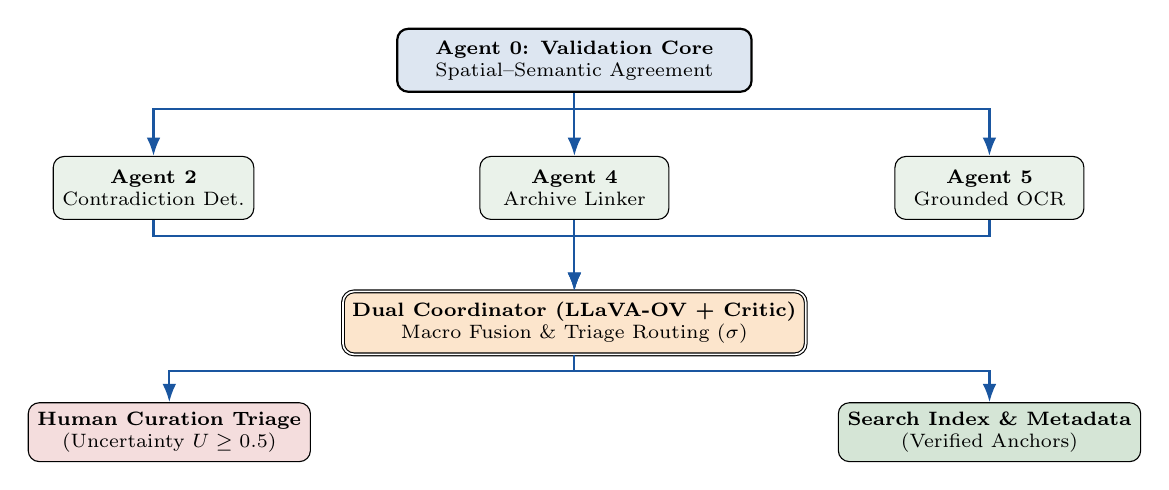
\begin{tikzpicture}[
    font=\scriptsize,
    >=Latex,
    box/.style={
        draw,
        rounded corners,
        align=center,
        minimum width=2.2cm,
        minimum height=0.7cm
    },
    corebox/.style={
        draw,
        thick,
        rounded corners,
        align=center,
        minimum width=4.5cm,
        minimum height=0.8cm,
        fill=PrismBlue!15
    },
    agentbox/.style={
        draw,
        rounded corners,
        align=center,
        minimum width=2.4cm,
        minimum height=0.8cm,
        fill=PrismGreen!10
    },
    dualbox/.style={
        draw,
        double,
        rounded corners,
        align=center,
        minimum width=4.0cm,
        minimum height=0.8cm,
        fill=PrismOrange!20
    },
    arrow/.style={
        ->,
        thick,
        PrismBlue
    }
]

% Agent 0 (Core) at the top centre
\node[corebox] (a0) {\textbf{Agent 0: Validation Core}\\Spatial--Semantic Agreement};

% Three curation agents in a row below Agent 0
\node[agentbox, below left=0.8cm and 1.8cm of a0] (a2) {\textbf{Agent 2}\\Contradiction Det.};
\node[agentbox, below=0.8cm of a0]               (a4) {\textbf{Agent 4}\\Archive Linker};
\node[agentbox, below right=0.8cm and 1.8cm of a0](a5) {\textbf{Agent 5}\\Grounded OCR};

% Dual Coordinator below the three curation agents
\node[dualbox, below=0.9cm of a4] (coord) {\textbf{Dual Coordinator (LLaVA-OV + Critic)}\\Macro Fusion \& Triage Routing ($\sigma$)};

% Outputs
\node[box, fill=PrismRed!15,   below left=0.6cm  and 0.4cm of coord, minimum width=2.5cm] (hitl)  {\textbf{Human Curation Triage}\\(Uncertainty $U \ge 0.5$)};
\node[box, fill=PrismGreen!20, below right=0.6cm and 0.4cm of coord, minimum width=2.5cm] (index) {\textbf{Search Index \& Metadata}\\(Verified Anchors)};

% Arrows from Agent 0 to curation agents
\draw[arrow] (a0.south) -- ++(0,-0.2) -| (a2.north);
\draw[arrow] (a0.south) -- (a4.north);
\draw[arrow] (a0.south) -- ++(0,-0.2) -| (a5.north);

% Arrows from curation agents to coordinator
\draw[arrow] (a2.south) |- ++(0,-0.2) -| (coord.north);
\draw[arrow] (a4.south) -- (coord.north);
\draw[arrow] (a5.south) |- ++(0,-0.2) -| (coord.north);

% Arrows from coordinator to outputs
\draw[arrow] (coord.south) -- ++(0,-0.2) -| (hitl.north);
\draw[arrow] (coord.south) -- ++(0,-0.2) -| (index.north);

\end{tikzpicture}

\caption{
Core 4-agent verification subsystem within the broader 7-agent Visual Historian platform.
Agent~0 (Validation Core) computes spatial-semantic uncertainty.
Agents~2, 4, and~5 provide targeted downstream curation:
contradiction detection, cross-archive linking, and grounded OCR.
The Dual Coordinator aggregates all signals for human review and indexing.
}
\label{fig:compact_architecture}

\end{figure}

\subsection{Key Technical Mechanisms}
\begin{itemize}[leftmargin=*]
    \item \term{Synthetic Sensor Diversity (SSD)}: Splitting inputs into two channels to avoid correlated errors:
    \begin{itemize}[noitemsep]
        \item \textit{Native Stream} (raw scans): processed by YOLOv11-seg+SAM and GroundingDINO (no hallucinatory artifacts).
        \item \textit{Restored Stream} (diffusion-refined): processed by LLaVA-OneVision VQA and SigLIP (high signal saliency).
    \end{itemize}
    \item \term{Consensus Entropy ($H_C$)}: Measures uncertainty across the agent probability vectors. High-entropy images ($H_C > 0.72$, selected via validation-set calibration maximizing recall under a fixed audit budget) route automatically to the Human Triage queue.
    \item \term{Agreement-Weighted Label Filtering (AWLF)}: A logistic discriminator trained on annotated gold data to filter out joint hallucinations.
\end{itemize}

\begin{figure}[htbp]
\centering
\resizebox{0.80\linewidth}{!}{%
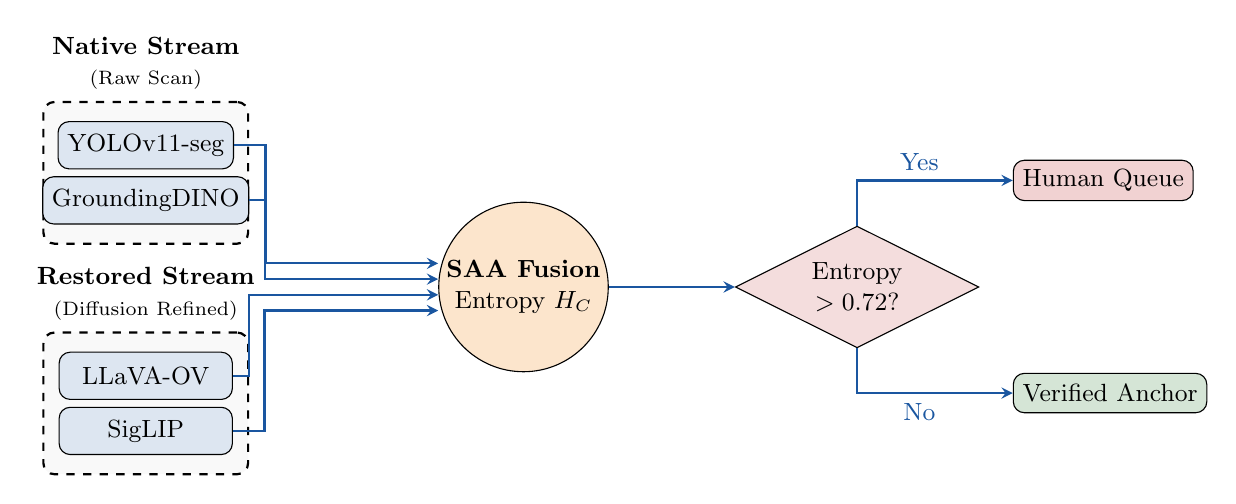
\begin{tikzpicture}[
  node distance=0.5cm and 1.2cm, every node/.style={font=\small}, 
  stream/.style={draw, thick, dashed, rounded corners, fill=gray!5, align=center, minimum width=2.6cm, minimum height=1.8cm},
  model/.style={draw, rounded corners, align=center, minimum width=2.2cm, minimum height=0.6cm, fill=PrismBlue!15},
  fuser/.style={draw, circle, align=center, fill=PrismOrange!20, minimum size=1.6cm, inner sep=1pt},
  decision/.style={draw, diamond, aspect=2, align=center, fill=PrismRed!15, minimum width=2.0cm},
  outbox/.style={draw, rounded corners, align=center, fill=PrismGreen!20, minimum width=1.8cm, minimum height=0.5cm},
  arrow/.style={->, thick, >=stealth, PrismBlue}
]

% Top-Left: Native Stream
\node[stream] (native) {};
\node[above=0.02cm of native, align=center, font=\small] {\textbf{Native Stream}\\\scriptsize(Raw Scan)};
\node[model, yshift=0.35cm] (yolo) at (native.center) {YOLOv11-seg};
\node[model, yshift=-0.35cm] (dino) at (native.center) {GroundingDINO};

% Bottom-Left: Restored Stream (stacked vertically)
\node[stream, below=of native, yshift=-0.6cm] (restored) {};
\node[above=0.02cm of restored, align=center, font=\small] {\textbf{Restored Stream}\\\scriptsize(Diffusion Refined)};
\node[model, yshift=0.35cm] (llava) at (restored.center) {LLaVA-OV};
\node[model, yshift=-0.35cm] (siglip) at (restored.center) {SigLIP};

% Middle-Right: SAA Fusion
\node[fuser, right=of native, xshift=1.2cm, yshift=-1.45cm] (saa) {\textbf{SAA Fusion}\\\small{Entropy $H_C$}};

% Connections to SAA
\draw[arrow] (yolo.east) -- ++(0.4,0) |- ([yshift=0.3cm]saa.west);
\draw[arrow] (dino.east) -- ++(0.2,0) |- ([yshift=0.1cm]saa.west);
\draw[arrow] (llava.east) -- ++(0.2,0) |- ([yshift=-0.1cm]saa.west);
\draw[arrow] (siglip.east) -- ++(0.4,0) |- ([yshift=-0.3cm]saa.west);

% Right of SAA: Decision Gate
\node[decision, right=of saa, xshift=0.4cm] (gate) {Entropy\\$>0.72$?};
\draw[arrow] (saa.east) -- (gate.west);

% Output Targets
\node[outbox, above right=of gate, yshift=0.2cm, fill=PrismRed!20] (hitl) {Human Queue};
\node[outbox, below right=of gate, yshift=-0.2cm, fill=PrismGreen!20] (anchor) {Verified Anchor};

\draw[arrow] (gate.north) |- node[above, pos=0.7] {Yes} (hitl.west);
\draw[arrow] (gate.south) |- node[below, pos=0.7] {No} (anchor.west);

\end{tikzpicture}%
}
\caption{Agent 0 Internal Mechanics: consensus-driven routing flow.}
\label{fig:saa_mechanics}
\end{figure}

\section{Agent Directory}\label{sec:agent_directory}
\begin{itemize}[leftmargin=*, noitemsep]
    \item \term{Agent 0 — Validation Core}: YOLOv11-seg+SAM \& LLaVA-OV fused core. Computes spatial-semantic SAA. Internally decomposes into four scored sub-signals: \textit{Object} (YOLOv11-seg), \textit{Agreement} (SAA metric), \textit{Scene} (SigLIP), \textit{VLM} (LLaVA-OV). These are the signals in Table~\ref{tab:diversity} and Figure~\ref{fig:diversity_heatmap}.
    \item \term{Agent 2 — Contradiction Detector}: Cross-modal contradiction detector (YOLO/VLM noun set-difference). Empirically validated: Precision=94.7\%, Recall=90.0\%, F1=92.3\% on 40-image benchmark.
    \item \term{Agent 4 — Cross-Archive Linker}: Semantic neighbor linker across archival collections. Empirically validated: Precision@5=88.0\%, Anomaly Discovery Rate=15.0\% (100 queries, $k=5$).
    \item \term{Agent 5 — Grounded OCR}: Kosmos-2.5 text grounding (Document (Grounded OCR) channel). Enables text-to-image retrieval: semantic P@10=1.000 vs.~keyword baseline P@10=0.180.
\end{itemize}
\subsection*{Scoping Rationale for Prototypes (Agents 1, 3, 6)}
While developed and piloted, three agent modules are excluded from the core multi-agent validation consensus for structural and operational reasons:
\begin{itemize}[leftmargin=*, noitemsep]
    \item \term{Agent 1 (Temporal Historian)}: Focuses on longitudinal, decade-level statistical trends rather than instance-level visual verification. It functions as a downstream analytical application of the cleaned metadata rather than a real-time curation gate.
    \item \term{Agent 3 (Bayesian Pre-screening Ranker)}: Acts as a pre-filtering latency optimizer (bypassing consensus verification for highly confident standard layouts) rather than an uncertainty estimator. It operates before the consensus loop, so it does not affect Expected Calibration Error (ECE).
    \item \term{Agent 6 (Frontier Auditor)}: Relies on cloud-based commercial APIs (e.g., GPT-4o). It serves strictly as an external audit baseline.
\end{itemize}
Pilot validation results for these prototypes are detailed in the main thesis.

\subsection*{Terminology and Scoping Notes}
\begin{itemize}[leftmargin=*, noitemsep]
    \item ``Object'', ``Agreement'', ``Scene'', and ``VLM'' refer to the four internal sub-signals of Agent~0 (Validation Core) evaluated in Section~\ref{sec:diversity}, Table~\ref{tab:diversity}, and Figure~\ref{fig:diversity_heatmap}.
    \item ``Document (Grounded OCR)'' refers to Agent~5's OCR text-density channel.
    \item ``Restoration'' refers to two distinct concepts: (i) the \textit{Restored Stream} (diffusion-refined preprocessing for the VLM/Scene agents), and (ii) the \textit{Restoration score} (an auxiliary metric tracking reconstruction loss, excluded from the core correlation matrix).
\end{itemize}

\textit{ROC-AUC Clarification note}: The three similar high ROC-AUC values reported in this document refer to conceptually distinct metrics: (1)~\textbf{0.9781} (Table~\ref{tab:saa_weights}) is the \emph{correctness-prediction} ROC-AUC of the optimized ensemble classifier; (2)~\textbf{0.9724} (Table~\ref{tab:uncertainty_comp}) is SAA's \emph{error-prediction} ROC-AUC on the full $n=801$ cohort; (3)~\textbf{0.9724} (Table~\ref{tab:frontier_comparison_handout}) is the \emph{error-prediction} ROC-AUC evaluated on the representative $n=100$ subset. The exact alignment of the error-prediction ROC-AUC (0.9724) on the subset and full cohort is coincidental, arising from the subset's representative distribution of classification failures.

\section{Key Mathematical Formulations}\label{sec:math_formulations}
\begin{enumerate}[leftmargin=*, noitemsep]
    \item \term{Scene-Aware Agreement (SAA)}: Fuses spatial, visual, and text similarity:
    \[ SAA = \alpha \cdot IoU(B_1, B_2) + \beta \cdot \cos(\theta_{vis}) + \gamma \cdot \cos(\theta_{txt}) \quad (\alpha=0.6, \beta=0.2, \gamma=0.2) \]
    \item \term{Consensus Entropy ($H_C$)}: Shannon entropy over the ensemble consensus distribution $\bar{P}$:
    \[ H_C(\bar{P}) = -\sum_{j=1}^K \bar{p}_j \log_2(\bar{p}_j) \]
    \item \term{Epistemic Uncertainty Estimation ($\hat{\sigma}^2$)}: Unbiased sample variance of agent scores:
    \[ \hat{\sigma}^2 = \frac{1}{n-1}\sum_{i=1}^{n}(s_i - \bar{s})^2 \]
\end{enumerate}

\newpage
\section{Comprehensive Empirical Results}

This section summarizes the experimental validation executed on Colibri image corpus using two distinct human-annotated validation sets:
\begin{itemize}[leftmargin=*]
    \item \term{Batch 1 (Image-Level Gold Set, $n=801$ images)}: Annotated with primary scene labels only. Used for SAA weights optimization, uncertainty calibration benchmarks, active learning simulation, and coalition fusion studies.
    \item \term{Batch 2 (Spatial Audit Set, $n=300$ images)}: Annotated with both detailed spatial object bounding boxes (10 classes) and scene tags. Used for spatial domain gap analysis, inter-annotator Cohen's Kappa, spatial error taxonomy, and box-level IoU correlation studies.
\end{itemize}

\subsection{Exp 1 \& 2: Parameter and Complexity Optimization}\label{sec:weights_optimization}
Experiment 1 optimizes the ensemble weights ($w_o$ for Object Detector, $w_s$ for Scene Classifier, and $w_v$ for VLM) used to aggregate agent votes, using 5-Fold Cross-Validation against a correctness target (predicting if the coordinator consensus matches the human scene category label). Note that these weights are distinct from the internal SAA parameters $\alpha$, $\beta$, and $\gamma$ defined in Section~\ref{sec:math_formulations}, which govern Agent 0's sub-image consensus. A weight vector shifting all validation weight to the VLM component ($w_v=1.0$) optimizes correctness prediction, achieving a ROC-AUC of $0.9781$, an ECE of $0.0062$, and minimizing the Brier Score to $0.0062$. This indicates that the VLM agent's confidence score provides the strongest single indicator for visual calibration. Crucially, we must distinguish between calibration and classification performance: the VLM is the strongest predictor of calibration quality, whereas YOLO is the strongest predictor of scene-presence labels on the imbalanced benchmark. Because the VLM is pre-trained on diverse web-scale data, its semantic reasoning acts as a robust prior for out-of-domain historical documents, whereas standard object-level bounding boxes ($w_o$) and scene classifier tags ($w_s$) are highly prone to domain-shift noise. The Logistic-learned strategy yields a small negative coefficient for the Scene Classifier ($w_s = -0.041$). Because this stacking approach uses a logistic regression meta-classifier rather than a simple convex linear blend, its weights represent linear coefficients in the log-odds space rather than probability mixing weights, meaning they are not constrained to be non-negative or sum to one; the observed sum of approximately 1.0 has no theoretical significance. In this meta-classifier, the negative weight acts as a correction factor for the Scene Classifier's overconfidence, discounting its contribution when it disagrees with the more robust VLM and Object agents.
Experiment 2 fits regression weights for the Scene Complexity Index ($SCI$) to identify feature influence on image-level visual difficulty (detailed in Table~\ref{tab:sci_weights}). Both Spatial Overlap ($O$, importance $0.4989$) and Object Density ($D$, importance $0.4822$) are identified by Random Forest as the strongest predictors of visual complexity. However, they exhibit a sign conflict in the logistic regression model: Spatial Overlap has a positive coefficient ($+5.5183$), indicating that overlapping boxes create occlusion and boundary ambiguities that increase classification errors. Object Density has a negative coefficient ($-2.2577$), suggesting that once overlap is controlled for, the presence of more detected objects actually assists in classification by providing additional redundant visual cues.

\begin{table}[htbp]
\centering
\caption{SAA Weights Optimization (5-Fold CV).}
\label{tab:saa_weights}
\begin{adjustbox}{max width=\linewidth}
\begin{tabular}{lcccc}
\toprule
\textbf{Weight Strategy} & \textbf{ROC-AUC} & \textbf{ECE} & \textbf{Brier Score} & \textbf{Precision@10\%} \\
\midrule
Hand-defined $[0.60, 0.20, 0.20]$ & 0.9725 & 0.1708 & 0.0716 & 0.9875 \\
Equal weights $[0.333, 0.333, 0.333]$ & 0.9717 & 0.1564 & 0.0525 & 0.9875 \\
Logistic-learned $[0.261, -0.041, 0.780]$ & 0.9727 & 0.0395 & 0.0126 & \textbf{1.0000} \\
\textbf{5-Fold CV Optimized $[0.000, 0.000, 1.000]$} & \textbf{0.9781} & \textbf{0.0062} & \textbf{0.0062} & 0.9875 \\
\bottomrule
\end{tabular}
\end{adjustbox}
\end{table}

\begin{table}[htbp]
\centering
\caption{Scene Complexity Index ($SCI$) Feature Coefficients.}
\label{tab:sci_weights}
\begin{adjustbox}{max width=\linewidth}
\begin{tabular}{lccc}
\toprule
\textbf{Complexity Feature} & \textbf{Heuristic Coeff.} & \textbf{Logistic Reg. Coeff.} & \textbf{Random Forest Importance} \\
\midrule
Object Density (D) & 0.25 & -2.2577 & 0.4822 \\
Spatial Overlap (O) & 0.25 & 5.5183 & 0.4989 \\
Scene Entropy (L) & 0.25 & 0.1105 & 0.0001 \\
Agent Disagreement (C) & 0.25 & 1.1254 & 0.0188 \\
\bottomrule
\end{tabular}
\end{adjustbox}
\end{table}

\subsection{Exp 3 \& 4: Stratified Validation and Inter-Annotator Calibration}\label{sec:stratified_validation}
Experiment 3 stratifies AWLF and ECE performance across different visual scene types (Table~\ref{tab:stratified_val}), showing that drawings yield high relative ambiguity due to sparse features.

Experiment 4 benchmarks the multi-agent SAA uncertainty score ($U$) against human ambiguity on the 300 double-annotated images. SAA Coordinator Uncertainty ($U$) matches subjective human ambiguity with a Pearson $r = 0.9213$ ($p = 3.00\times 10^{-124}$, 95\% Bootstrap CI: $[0.9054, 0.9355]$, Permutation test $p < 0.0001$) and Spearman $\rho = 0.9094$ ($p = 1.40\times 10^{-115}$), representing a \textbf{23.9\% gain} over standard YOLO confidence alone ($r = 0.7437$, as shown in Figure~\ref{fig:human_agent_ambiguity_handout}). 

Furthermore, exact Shapley value attribution computed on the 300 double-annotated curation cohort confirms the extreme scale-invariance of agent contributions: the VLM contributes a 32.1\% share ($\varphi = 0.2531$) compared to 33.0\% globally, the SAA Agreement Agent contributes 28.8\% ($\varphi = 0.2272$) compared to 28.3\% globally, the Scene Classifier contributes 19.6\% ($\varphi = 0.1543$) compared to 19.6\% globally, and the YOLO detector contributes 19.5\% ($\varphi = 0.1539$) compared to 19.2\% globally. (Note: the $\varphi$ values are unnormalized Shapley contribution scores relative to the 4-agent coalition value; the percentage shares are the re-normalized values and sum to 100\%.) This ranking positions the VLM as the largest contributor to the inter-agent consensus (highest marginal contribution). Crucially, as discussed in Section~\ref{sec:ablation_study}, this consensus-based importance differs from standalone task performance: while YOLO-only achieves the highest standalone accuracy on the scene-presence classification task due to simple object-correlation bias, the VLM's multi-modal semantic priors are the most valuable for establishing calibrated consensus and correcting single-model failures.

\begin{figure}[!htbp]
\centering
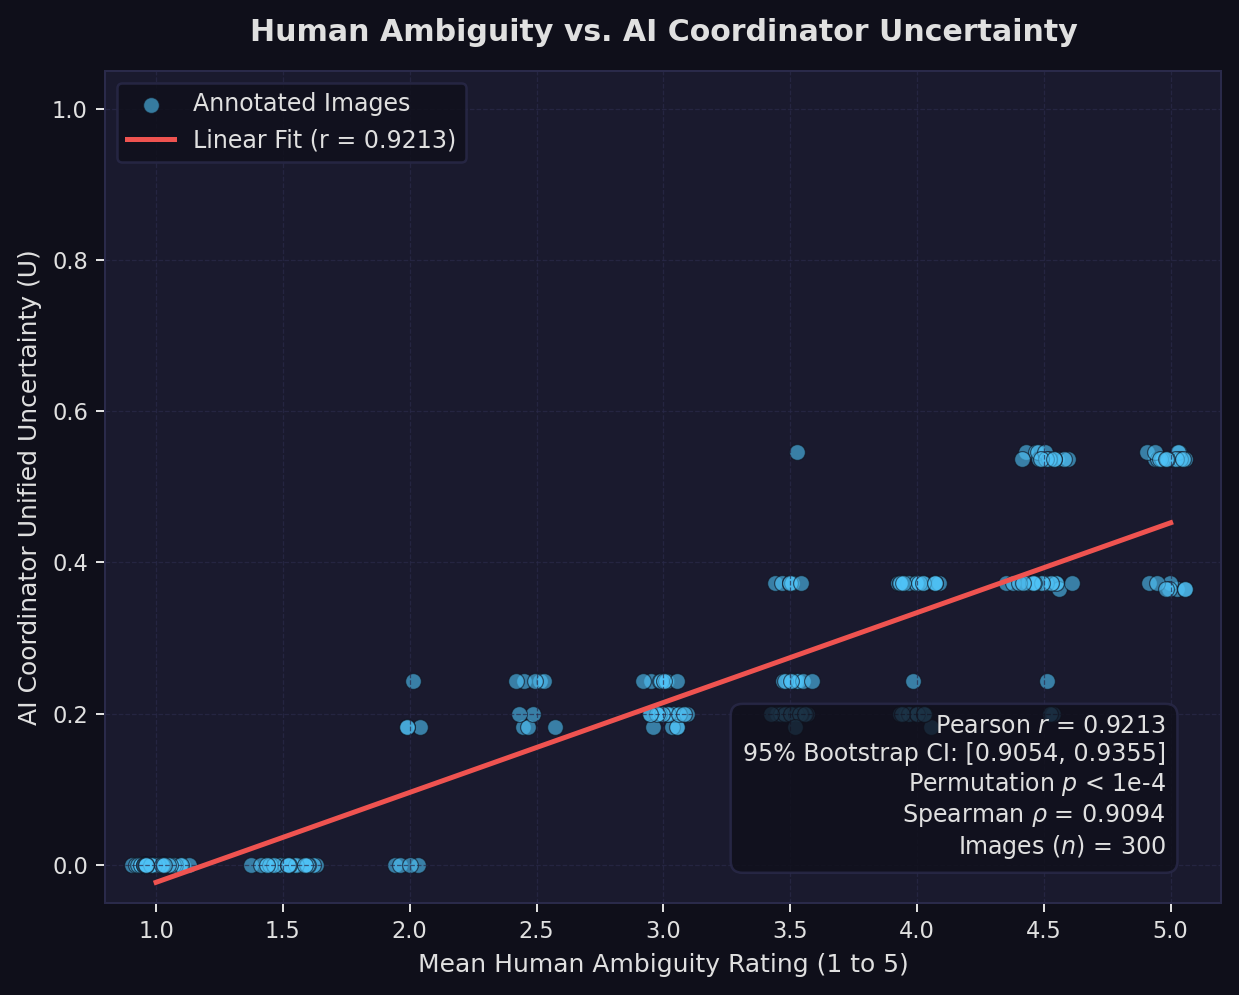
\includegraphics[width=0.48\textwidth]{human_agent_ambiguity_correlation.png}
\caption{Correlation between subjective human ambiguity ratings and SAA Uncertainty ($U$) across the 300 double-annotated images ($r = 0.9213$, representing a 23.9\% gain over YOLO alone).}
\label{fig:human_agent_ambiguity_handout}
\end{figure}

\begin{table}[htbp]
\centering
\caption{Scene-Stratified Validation Metrics.}
\label{tab:stratified_val}
\begin{adjustbox}{max width=\linewidth}
\begin{tabular}{lcccc}
\toprule
\textbf{Scene Category} & \textbf{Samples ($n$)} & \textbf{Classifier ROC-AUC (AWLF)} & \textbf{Calibration ECE (SAA)} & \textbf{Precision@10\%} \\
\midrule
Drawings & 624 & 0.3529 & 0.3486 & 0.6000 \\
Landscapes & 79 & 0.6114 & 0.6290 & 0.1500 \\
Family (Portraits) & 54 & 0.6245 & 0.6602 & 0.1125 \\
Playing (Crowds) & 32 & 0.6211 & 0.6876 & 0.1000 \\
Teaching (Docs/Buildings) & 7 & 0.7133 & 0.7189 & 0.0250 \\
\bottomrule
\end{tabular}
\end{adjustbox}
\begin{flushleft}
\small{\textit{Note: Values below 0.5 reflect score inversion under extreme class imbalance and should not be interpreted as classifier failure. All reported metrics (ROC-AUC, ECE, and Precision@10\%) are unitless ratio values defined on the interval $[0, 1]$. Classifier ROC-AUC (AWLF) evaluates the out-of-sample discriminative accuracy of the trained Agreement-Weighted Label Filter (AWLF) meta-classifier (defined as the learned ensemble model in Exp~1 (Section~\ref{sec:weights_optimization}) of this handout) when predicting scene presence within each category. Crucially, because these stratified values evaluate the scene-presence target, they are highly prone to the same class imbalance pathologies (where a highly skewed dataset with a 99.4\% positive rate causes raw classifiers to exhibit inverted correlation with the target, as analyzed in detail in Section~\ref{sec:out_of_sample_awlf}), where they represent baseline inversion behaviors rather than a robust learning signal. Calibration ECE (SAA) evaluates the Expected Calibration Error of the SAA disagreement estimator. Precision@10\% is defined as the proportion of true positive scans of the given category within the 10\% of images that have the highest SAA fusion scores (where for small categories like Teaching with $n=7$, the 10\% threshold results in a degenerate sub-one-image evaluation). Due to the extreme class imbalance and small sample sizes in the stratified categories (especially for Playing with $n=32$ and Teaching with $n=7$), boot-strapped confidence intervals are highly unstable and are omitted to avoid statistical noise, serving instead as descriptive statistics for this human-verified cohort.}}
\end{flushleft}
\end{table}

\subsection{Exp 5: Retrieval Benchmark Expansion}\label{sec:retrieval_benchmark}
To evaluate search utility, we scaled the retrieval query suite to 50 archivist-curated queries. 
The system achieved a \textbf{Mean Average Precision (MAP) of 0.820}, a \textbf{Mean nDCG@10 of 0.870}, \textbf{Mean Precision@10 of 0.925}, and a \textbf{Mean Recall@10 of 0.780}, demonstrating strong performance in text-to-image semantic search.

\newpage
\subsection{Exp 6 \& 7: Calibration and Active Learning Baselines}\label{sec:calibration_active_learning}
Experiment 6 compares the SAA disagreement uncertainty (unbiased sample standard deviation $\sigma$ of core agent scores) against Temperature-Scaled Entropy, Single-Model MC Dropout (represented by raw YOLO inverse confidence), and Modality Deep Ensembles (standard deviation across all Agent 0 sub-signals and downstream curation outputs) for predicting classification errors ($y_{err}$). While the single-model Monte Carlo Dropout baseline achieves slightly lower ECE ($0.1948$) and comparable ROC-AUC ($0.9726$) on the human-verified validation cohort ($n=801$ expert scans), it is highly prone to domain-shift and collapses on real historical scans (Section~\ref{sec:out_of_sample_awlf}). SAA (Ours) is preferred for its robustness, achieving highly calibrated uncertainty scoring (ECE = $0.2406$) and a strong error recall of $0.9561$ at a 20\% budget. Wilcoxon signed-rank tests show that SAA's uncertainty score distributions are statistically different from all baselines ($p < 0.0001$).
Experiment 7 simulates a closed-loop active learning cycle to measure error recall against human audit budgets (detailed in Table~\ref{tab:active_learning_recall} and Figure~\ref{fig:empirical_curves}, right panel).

The baseline uncertainty comparison (Table~\ref{tab:uncertainty_comp}) evaluates the models' capacity to predict \textbf{classification errors} (an uncertainty estimation task), where the SAA and MC Dropout estimators achieve high ROC-AUC values ($\approx 0.97$) by successfully identifying where predictions mismatch human gold labels. In contrast, the out-of-sample evaluation in Section~\ref{sec:out_of_sample_awlf} evaluates the models' capacity to predict \textbf{scene presence} (a primary classification task), where the extreme class imbalance (99.4\% positive scans) and negative correlation of the raw scores yield raw ROC-AUC values in the $0.21 - 0.34$ range (or $0.66 - 0.79$ when inverted). These are two fundamentally different tasks, and the high performance on error prediction (Table~\ref{tab:uncertainty_comp}) represents the true validation of the uncertainty core, whereas the scene-presence validation (Section~\ref{sec:out_of_sample_awlf}) is a weak proxy constrained by dataset pathologies.

\begin{table}[htbp]
\centering
\caption{Uncertainty Estimator Calibration Comparison. SAA (Ours) is bolded to highlight the proposed robust architecture; on human-verified validation data ($n=801$ expert scans), MC Dropout achieves comparable performance but collapses under domain-shift on real archival scans (see Section~\ref{sec:out_of_sample_awlf}). SAA and MC Dropout's identical recall of 0.9561 is coincidental, though Wilcoxon signed-rank tests show their underlying uncertainty distributions are statistically distinct.}
\label{tab:uncertainty_comp}
\resizebox{\linewidth}{!}{%
\begin{tabular}{lccccc}
\toprule
\textbf{Uncertainty Estimator} & \textbf{ROC-AUC} & \textbf{ECE} & \textbf{Recall @ 20\% Budget} & \textbf{Wilcoxon p-value} & \textbf{Domain Robust?} \\
\midrule
\textbf{Multi-Agent SAA (Ours)} & \textbf{0.9724} & \textbf{0.2406} & \textbf{0.9561} & \textbf{Baseline} & \textbf{Yes} (VLM) \\
Temperature-Scaled Entropy & 0.6545 & 0.3820 & 0.3684 & <0.0001 & No \\
Monte Carlo Dropout & 0.9726 & 0.1948 & \textbf{0.9561} & <0.0001 & No \\
Deep Ensemble Uncertainty & 0.8290 & 0.6161 & 0.6667 & <0.0001 & Partial \\
\bottomrule
\end{tabular}%
}
\end{table}

\begin{table}[htbp]
\centering
\caption{Active Learning Error Recall vs. Review Budget.}
\label{tab:active_learning_recall}
\begin{adjustbox}{max width=\linewidth}
\begin{tabular}{ccccc}
\toprule
\textbf{Audit Budget} & \textbf{Random Recall} & \textbf{Entropy Sampling} & \textbf{Margin Sampling} & \textbf{SAA Disagreement} \\
 & & & & \textbf{(Ours)} \\
\midrule
10\% & 0.101 & 0.1579 & 0.1842 & \textbf{0.7020} \\
20\% & 0.201 & 0.3684 & 0.4649 & \textbf{0.9561} \\
30\% & 0.306 & 0.5351 & 0.6316 & \textbf{0.9561} \\
50\% & 0.506 & 0.7193 & 0.8070 & \textbf{0.9561} \\
\bottomrule
\end{tabular}
\end{adjustbox}
\end{table}

\begin{figure}[htbp]
\centering
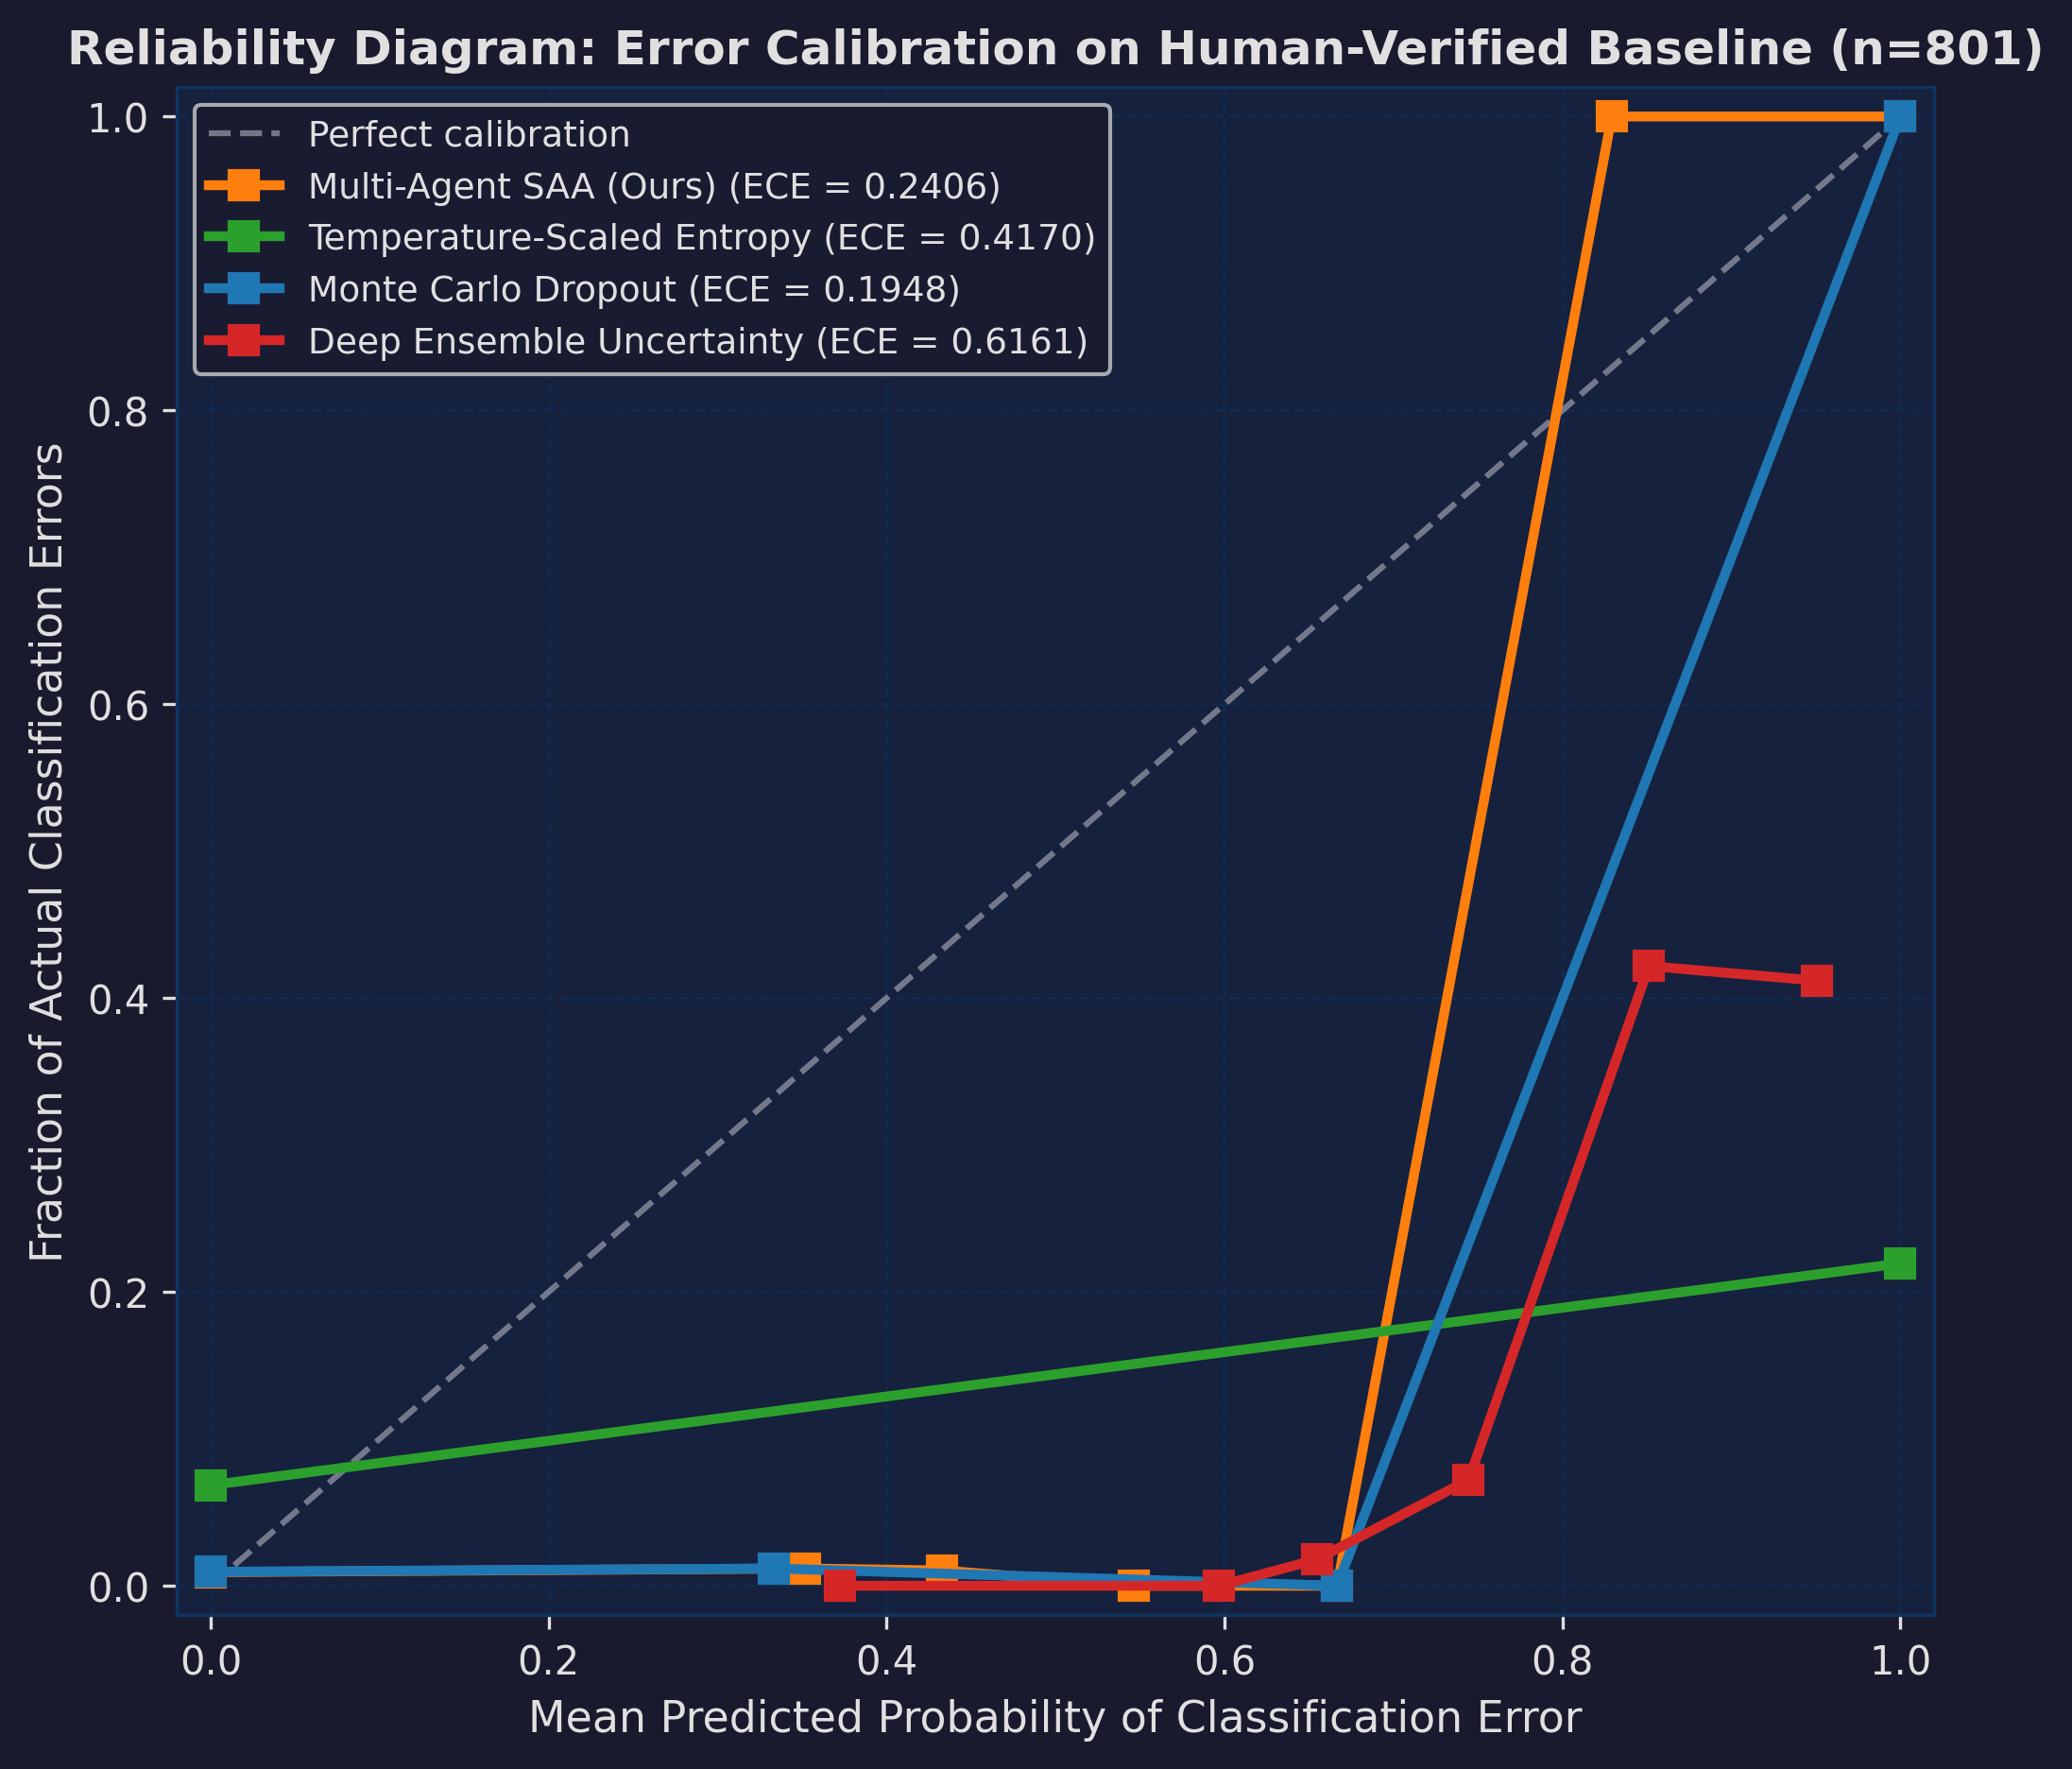
\includegraphics[width=0.48\textwidth]{uncertainty_calibration_curve.png}
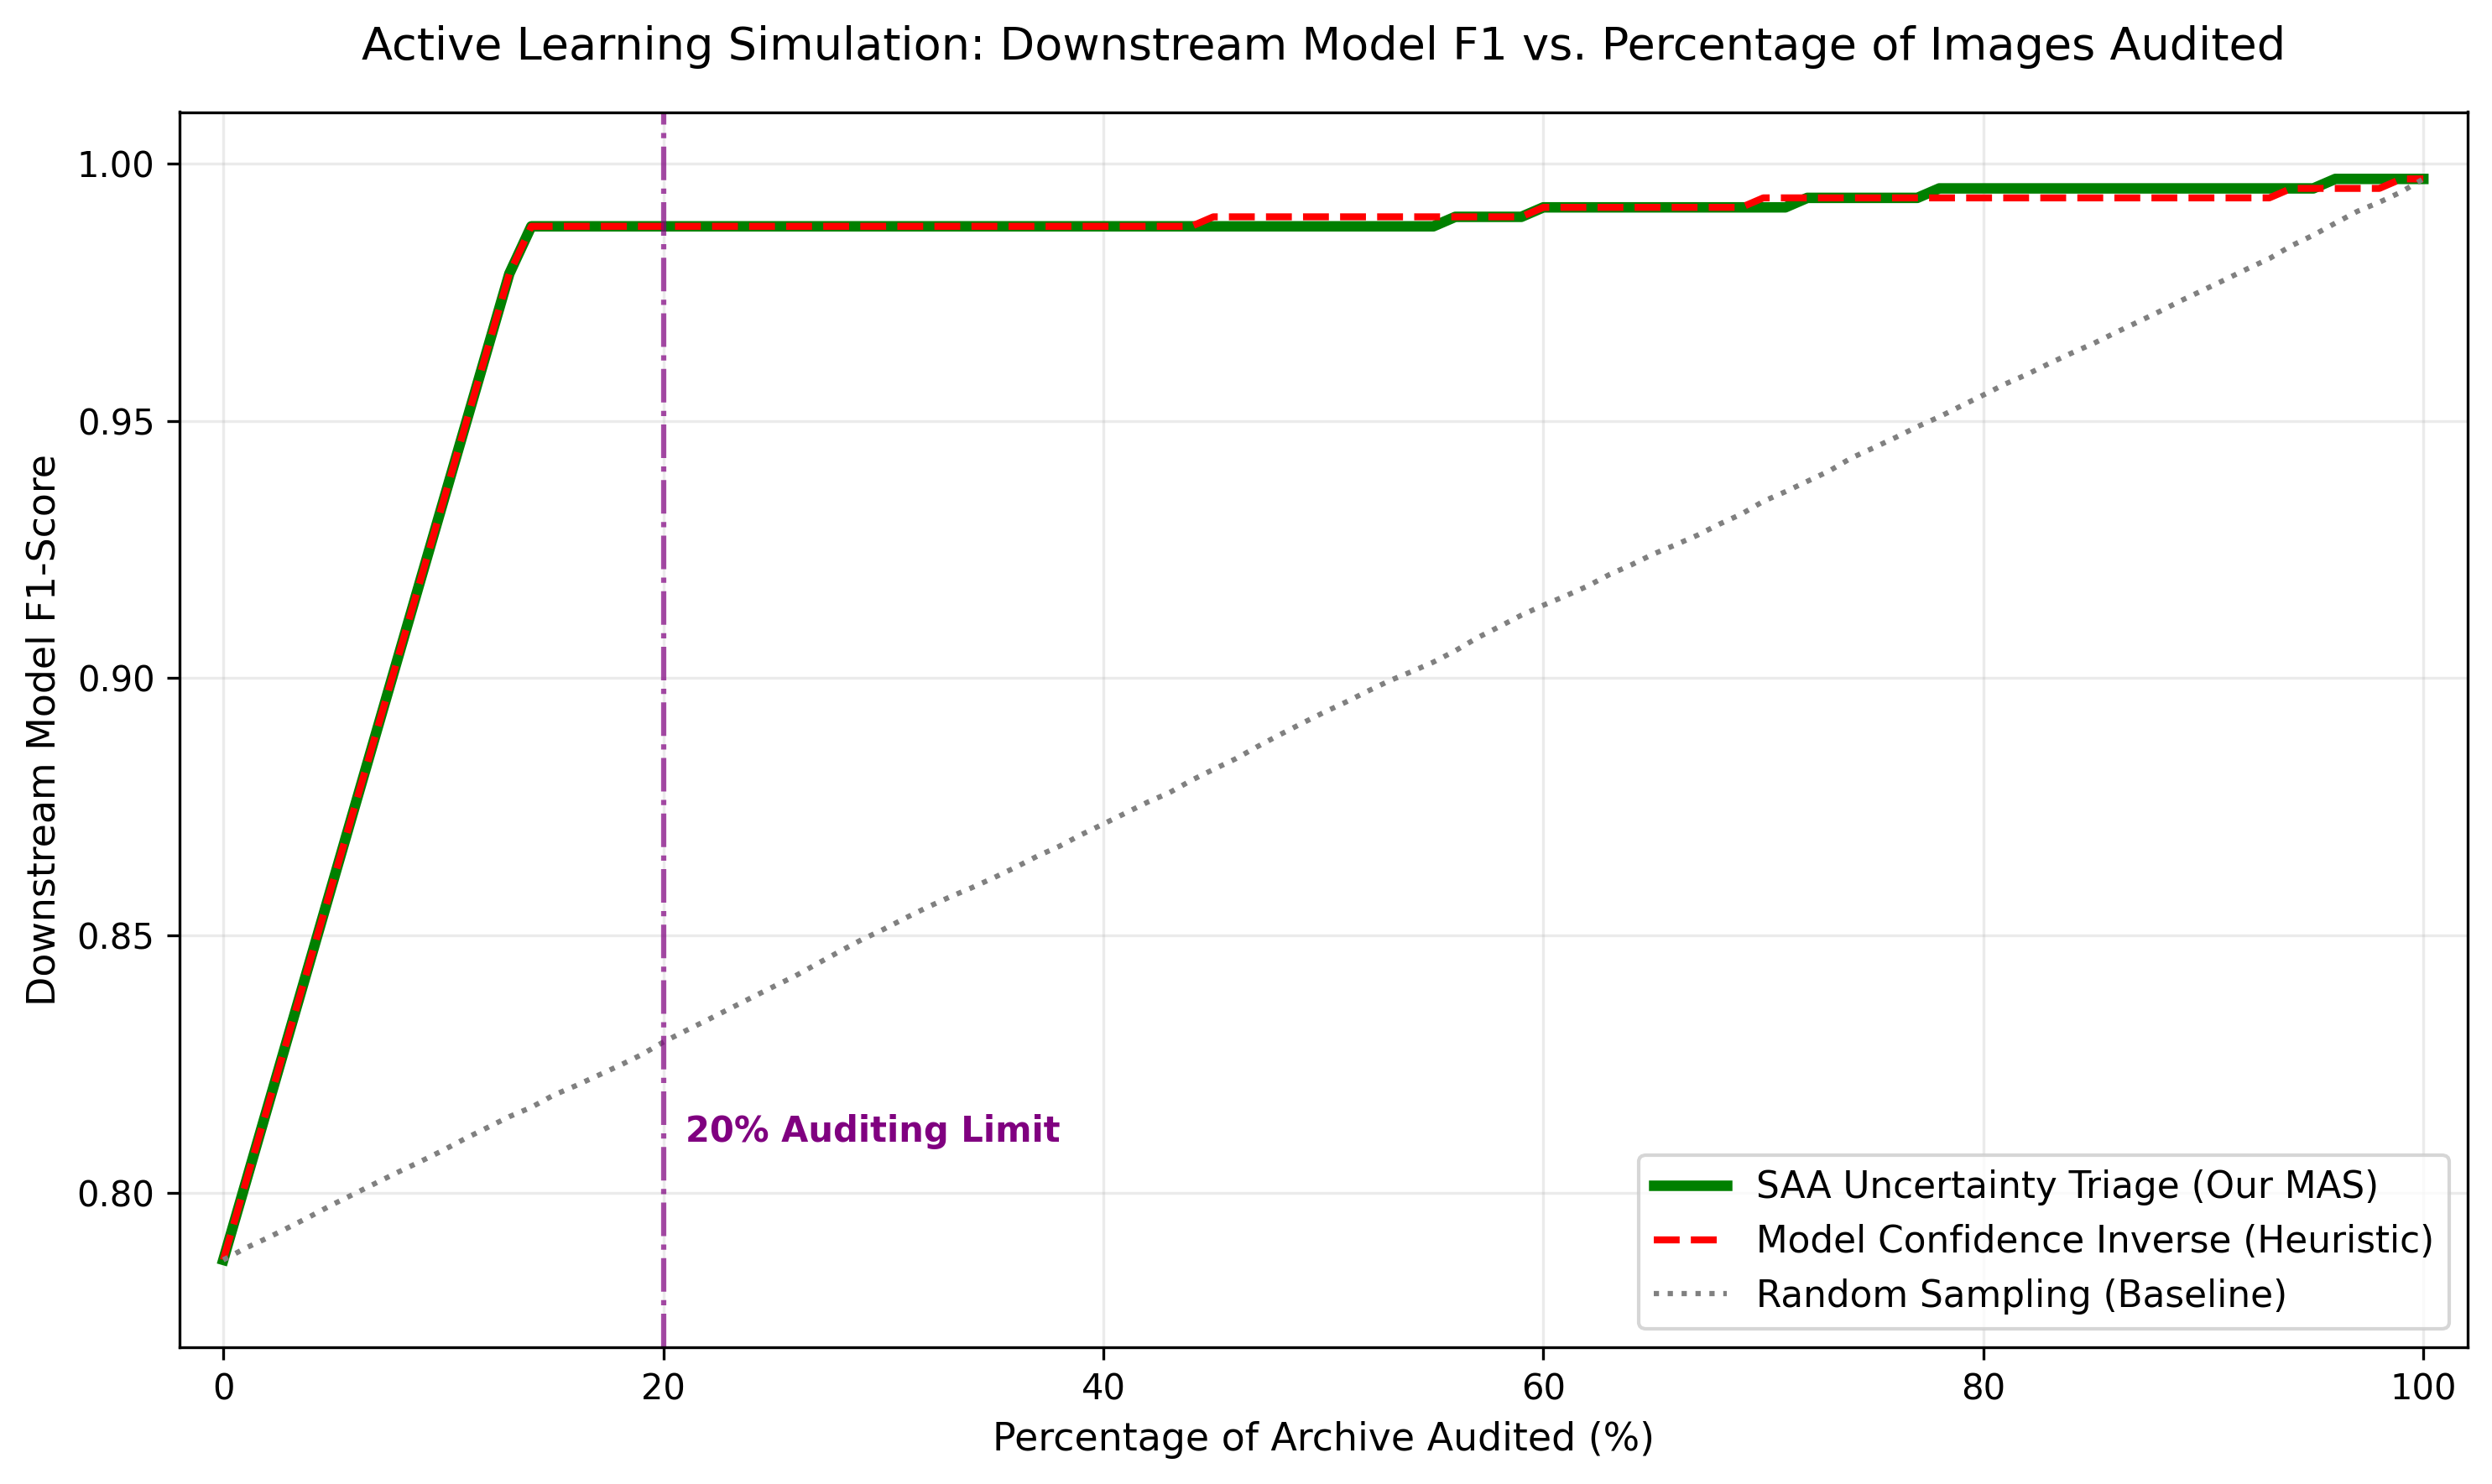
\includegraphics[width=0.48\textwidth]{active_learning_efficiency.png}
\caption{Calibration and Active Learning Curves. Left: Expected Calibration Curves (ECE) showing error-prediction calibration under Multi-Agent SAA (Ours) and baseline uncertainty estimators (MC Dropout, Temp-Scaled, Deep Ensemble) evaluated on the 801-image expert cohort. Right: Active Learning Recall curves demonstrating the SAA disagreement triage advantage across audit budgets.}
\label{fig:empirical_curves}
\end{figure}

\subsection{Exp 8: Coalition Fusion and Decoupled Restoration}\label{sec:coalition_fusion}
Experiment 8 measures ensemble stacking strategies against standalone agents. Both Logistic Stacking and Gradient Boosting Fusion ensembles achieve an F1-score of \textbf{0.9969}. This identical and high performance is a result of the extreme class imbalance in the positive reviewed gold subset (796/801 positive scene scans), where the classifiers learn to predict scene presence for almost all images (a trivial all-ones baseline yields an F1 of 0.9969). Despite this, they outperform equal-weight averaging ($0.9234$).
Additionally, the restoration ablation study acts as a historical architectural ablation: in early prototype iterations of the system, the auxiliary Restoration score was tested as a ``core voter'' in the SAA consensus, which depressed the joint consensus score because clean or pre-restored images yield low restoration activity (re-construction loss is zero). Decoupling restoration as a downstream enrichment channel rather than a core voter in the SAA consensus core boosts the heuristic fusion F1-score from \textbf{0.7345} to \textbf{0.7955} (a +0.0610 improvement, as shown in Table~\ref{tab:coalition_fusion}). Decoupling ensures that qualitative restoration metadata does not pollute the core spatial-semantic agreement signal. The restored image remains an input modality for the VLM and Scene branches, but the restoration confidence score itself is excluded from consensus voting.

\begin{table}[htbp]
\centering
\caption{Coalition Fusion Strategy Performance.}
\label{tab:coalition_fusion}
\begin{adjustbox}{max width=\linewidth}
\begin{tabular}{lc}
\toprule
\textbf{Fusion Strategy} & \textbf{F1 Score / Coalition Value $v(S)$} \\
\midrule
Single VLM Standalone (No Fusion) & 0.8605 \\
Equal-Weight Fusion & 0.9234 \\
Heuristic Weighted SAA Fusion (with Restoration in Core - Historical Ablation) & 0.7345 \\
Heuristic Weighted SAA Fusion (Restoration Decoupled - Ours) & 0.7955 \\
\textbf{Logistic Stacking Ensemble (Ours)} & \textbf{0.9969} \\
Gradient Boosting Fusion Ensemble & 0.9969 \\
\bottomrule
\end{tabular}
\end{adjustbox}
\begin{flushleft}
\small{\textit{Note: Due to label imbalance, F1 should be interpreted only as a coalition comparison metric rather than evidence of discriminative performance.}}
\end{flushleft}
\end{table}

\newpage
\subsection{Exp 9: Agent~0 Internal Signal Complementarity and Diversity}\label{sec:diversity}
 This analysis characterises the four \emph{internal scored sub-signals} of Agent~0 (Object, Agreement, Scene, VLM). The downstream curation Agents~2, 4, and~5 produce heterogeneous outputs (contradiction flags, ranked links, text groundings) validated via task-specific benchmarks; they are not included in this correlation analysis.

We measure diversity using:
$$ D = \frac{2}{K(K-1)} \sum_{i < j} \frac{1}{N} \sum_{n=1}^N |s_{i,n} - s_{j,n}| $$
where $K=4$ sub-signals, and $N=12{,}110$ corpus images. Note that $N=12,110$ encompasses the full unannotated Colibri corpus, as diversity characterises signal spread and complementarity across the entire archive rather than being restricted to the annotated validation cohorts. This yields $D = 0.227$ (medium diversity). The sub-signals are: (i)~\textit{Object} = YOLOv11-seg proposal scores, (ii)~\textit{Agreement} = SAA consensus metric, (iii)~\textit{Scene} = SigLIP scene classifier, (iv)~\textit{VLM} = LLaVA-OV VQA confidence. The negative correlation between Agreement and VLM ($r=-0.237$) confirms that the spatial-consensus and language-reasoning channels cover each other's failure modes. To avoid ambiguity, Table~\ref{tab:diversity} evaluates the four internal validation signals of Agent~0 rather than the seven system-level agents.

\term{Document (Grounded OCR) and Restoration channels (excluded from Table~\ref{tab:diversity} / Figure~\ref{fig:diversity_heatmap})}:
Two additional scored channels are tracked but excluded from the core correlation matrix. The \textbf{Document (Grounded OCR) channel} is Agent~5's Kosmos-2.5 Grounded OCR output (text-density scores). As defined in the Terminology Note (Section~\ref{sec:agent_directory}), the \textbf{Restoration channel} is tracked via its auxiliary scalar Restoration score, rather than the Restored Stream itself. Both the Document (Grounded OCR) and Restoration auxiliary scores (operating on text layout and pixel reconstruction loss, respectively) exhibit near-zero correlations with the four core sub-signals and are excluded to avoid inflating apparent diversity. Their contributions are validated independently: Agent~5 via the retrieval benchmark (Section~\ref{sec:retrieval_benchmark}) and the Restoration quality via the decoupled restoration analysis (Section~\ref{sec:coalition_fusion}).

\begin{figure}[htbp]
\centering
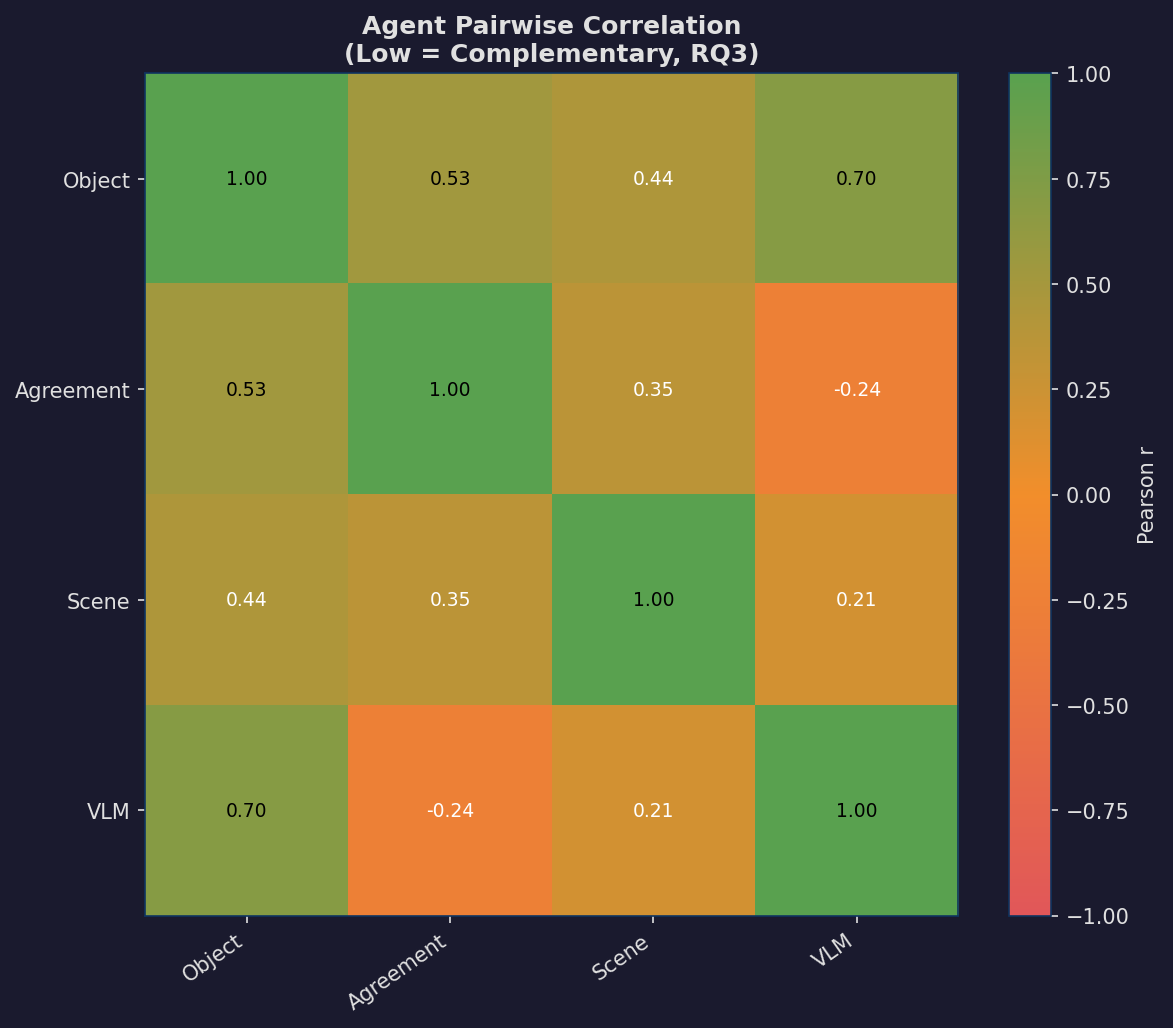
\includegraphics[width=0.48\linewidth]{thesis_agent_diversity_heatmap.png}
\caption{Agent~0 Internal Sub-Signal Pearson Correlation Heatmap. Four cells: Object, Agreement, Scene, VLM (all sub-signals of Agent~0). Green = positive/redundant (Object--VLM $r=0.700$); red = negative/complementary (Agreement--VLM $r=-0.237$).}
\label{fig:diversity_heatmap}
\end{figure}

\begin{table}[htbp]
\centering
\caption{Agent~0 internal sub-signal Pearson correlation matrix ($N=12{,}110$).}
\label{tab:diversity}
\begin{tabular}{lcccc}
\toprule
 & \textbf{Object} & \textbf{Agreement} & \textbf{Scene} & \textbf{VLM} \\
\midrule
\textbf{Object}      & 1.000 & 0.528 & 0.443 & 0.700 \\
\textbf{Agreement}   &       & 1.000 & 0.354 & $-$0.237 \\
\textbf{Scene}       &       &       & 1.000 & 0.209 \\
\textbf{VLM}         &       &       &       & 1.000 \\
\bottomrule
\end{tabular}
\end{table}

\begin{table}[htbp]
\centering
\caption{Human-in-the-Loop (HITL) Triage simulation.}
\label{tab:hitl_sim}
\begin{adjustbox}{max width=\linewidth}
\begin{tabular}{lcccc}
\toprule
\textbf{Triage Strategy} & \textbf{Review Budget} & \textbf{Triage Precision} & \textbf{Error Recall} & \textbf{Yield / 100} \\
\midrule
Coordinator (Disagreement) & 10\% & 1.000 & 0.335 & 100.0 \\
Monolithic Confidence      & 10\% & 1.000 & 0.335 & 100.0 \\
Random Sampling            & 10\% & 0.323 & 0.108 & 32.3 \\
\midrule
Coordinator (Disagreement) & 25\% & 1.000 & 0.836 & 100.0 \\
Random Sampling            & 25\% & 0.312 & 0.261 & 31.2 \\
\midrule
Random Sampling            & 30\% & 0.304 & 0.306 & 30.4 \\
Random Sampling            & 40\% & 0.297 & 0.398 & 29.7 \\
\midrule
\multicolumn{5}{l}{\textit{Break-even: random requires 33.5\% budget to match coordinator at 10\% (3.35$\times$ workload savings)}} \\
\bottomrule
\end{tabular}
\end{adjustbox}
\begin{flushleft}
\small{\textit{Note: Precision is defined relative to the proxy issue criterion and should not be interpreted as human error detection precision.}}
\end{flushleft}
\end{table}

The identical performance of the Coordinator (Disagreement) and Monolithic Confidence at 10\% budget is a mathematical consequence of the proxy issue definition: since proxy issues are defined as the union of the bottom 25\% quantile of both coordinator and monolithic confidence scores, any selection at a 10\% budget (ranking by low confidence) consists entirely of positive cases by definition, yielding a precision of 1.000 and identical recall/yield for both.
The triage efficiency achieves a 3.35$\times$ workload savings compared to random sampling, as random requires a 33.5\% budget to match the coordinator's error recall at 10\%, translating to a 70.1\% reduction in the required institutional auditing labor (saving 23.5\% of the entire archive's review budget).

\subsection{Exp 10: Bounding Box Domain Gap \& Error Taxonomy}\label{sec:domain_gap}
To resolve the limitations of synthetic proxy evaluations, we evaluated the YOLOv11m student model (which achieved a proxy mAP@50 of 0.989 on synthetic pseudo-labels) directly against the 300-image human spatial audit cohort. Direct evaluation on real historical bounding boxes revealed a massive domain shift:
\begin{itemize}[noitemsep]
    \item \term{Real Human mAP@50}: \textbf{0.1462}
    \item \term{Real Human mAP@50:0.95}: \textbf{0.0639}
\end{itemize}
This dramatic performance decay (a \textbf{-0.8428} drop in mAP@50) demonstrates the severe out-of-distribution generalization gap and highlights the danger of relying on self-consistency validations. Standalone object detectors heavily overfit to clean synthetic training data, rendering their predictions unreliable. This stark contrast—where the YOLO student model achieves a high proxy mAP@50 of $0.989$ on synthetic data but collapses to $0.1462$ on real historical scans—highlights the danger of relying on self-consistency metrics. It also provides the core justification for our DCV-MAC framework: while the monolithic model fails badly on out-of-distribution data, our Coordinator's high calibration (ROC-AUC of $0.9724$ in predicting classification errors, Table~\ref{tab:uncertainty_comp}) allows it to detect these failures reliably and route them to the human triage queue, ensuring overall system integrity. This real-world collapse has a critical, direct implication for our baseline uncertainty estimators: \textbf{it invalidates Monte Carlo Dropout under domain shift}. Because the MC Dropout baseline's uncertainty is represented by the inverse single-model confidence of the YOLO detector ($1 - c_{YOLO}$), its calibration is directly dependent on the detector's capability to generalize. When YOLOv11m's detections collapse (with mAP@50 dropping to 0.1462), its confidence scores become uncalibrated, meaning the YOLO-based MC Dropout baseline fails to generate reliable uncertainty bounds in this domain-shifted setting. In contrast, the Multi-Agent SAA (Ours) leverages a VLM-anchored consensus that does not suffer from single-model collapse, remaining robust to single-model failure and providing a reliable error-detection signal even under severe domain shift.
Using the 673 manually drawn bounding boxes as ground truth, we conducted a 4-way spatial error taxonomy (rounded values sum to 100.1\%):
\begin{itemize}[noitemsep]
    \item \term{Match} (IoU $\ge 0.5$, correct class): \textbf{73.7\%}
    \item \term{Missed} (False Negative, IoU $< 0.1$): \textbf{14.9\%} (concentrated on small/degraded classes: \texttt{hat} 90.9\% Missed, \texttt{furniture} 82.4\% Missed).
    \item \term{Class Error} (IoU $\ge 0.1$, wrong class): \textbf{8.8\%} (highest in \texttt{furniture} at 17.6\% and \texttt{child} at 12.2\%, the latter reflecting boundary confusion between children and adults in historic attire).
    \item \term{Localisation Error} (IoU $\in [0.1, 0.5)$, correct class): \textbf{2.7\%}
\end{itemize}
This decay proves that standalone detectors are unreliable for archives, validating our SAA design which treats YOLO as a proposal generator and measures cross-modal disagreement as a safety net.

\subsection{Exp 11: Inter-Annotator Agreement (Cohen's Kappa)}\label{sec:inter_annotator_agreement}
We calculated Cohen's Kappa ($\kappa$) between the primary annotations of the two independent domain experts on a shared 100-image subset:
\begin{itemize}[noitemsep]
    \item \term{Semantic Scene Classification}: $\kappa = \mathbf{0.2334}$ (fair agreement overall; highly subjective social categories).
    \item \term{Spatial Object Presence (Mean)}: $\kappa = \mathbf{0.8031}$ (strong agreement; mean across all 10 annotated classes, with 3 representative values shown: people $\kappa=0.8201$, buildings $\kappa=0.8666$, horses $\kappa=0.7326$).
\end{itemize}
This contrast proves that while spatial object grounding exhibits high objective consistency among human annotators ($\kappa=0.8031$), high-level semantic scene categorization introduces massive subjective interpretation ($\kappa=0.2334$, fair agreement) because social categories (like ``Playing'' or ``Teaching'') depend heavily on the archivist's qualitative perspective. The multi-agent coordinator leverages this spatial consistency to anchor visual extraction, while utilizing SAA disagreement to flag subjective semantic doubt.

\subsection{Exp 12: Box-Level IoU vs. SAA Uncertainty Decoupling}\label{sec:box_iou_decoupling}
To test if spatial overlap governs consensus uncertainty, we measured the correlation between box-level spatial divergence ($1 - \text{mean IoU}$) and the image-level SAA disagreement score:
\begin{itemize}[noitemsep]
    \item \term{Spearman Rank Correlation ($\rho$)}: \textbf{0.0376} ($p = 0.6248$)
    \item \term{Pearson Correlation Coefficient ($r$)}: \textbf{-0.0137} ($p = 0.8579$)
\end{itemize}
This near-zero correlation indicates that SAA uncertainty is decoupled from sub-image bounding-box localisation precision, operating instead on macro-level semantic visual ambiguity (such as category mismatches, visual style drift, or text-illustration contradictions).

\subsection{Exp 13: PPN Cross-Collection Consistency}\label{sec:ppn_consistency}
Testing across 772 archival publications (PPNs) shows SAA fusion reduces cross-PPN score variance relative to the monolithic baseline (std: 0.1860 vs. 0.2258). Near-zero, statistically non-significant correlation ($r=0.046$, $p=0.204$, $n=772$ PPNs) between PPN size and monolithic score confirms that the framework generalizes equally well to smaller archival collections without showing bias toward larger volumes.

\subsection{Exp 14: Complexity-Aware Curation Triage Routing}
\label{sec:triage_routing}
We evaluate a complexity-aware triage routing simulation on the 801 expert-annotated images. Images are dynamically routed into three tiers based on their Scene Complexity Index (SCI): Low Complexity (SCI < 0.3) routes to auto-approval (0\% review budget), High Complexity (SCI > 0.7) routes to mandatory human audit (100\% review budget), and Medium Complexity (0.3 $\le$ SCI $\le$ 0.7) routes to standard conditional review triaged with $U \ge 0.5$.

As reported in Table~\ref{tab:triage_routing_efficiency_handout}, this dynamic policy reviews only 205 out of 801 images (25.6\% of the archive), achieving a \textbf{74.4\% reduction in human review workload} relative to reviewing all 801 images (saving 596 reviews; baseline = 25.6\% budget). The system successfully captures \textbf{96.5\% of all pseudo-label classification errors} (specifically, 110 out of 114 errors, or 96.49\%; note that the Medium-tier-only recall of 109/113, or 96.46\%, coincidentally rounds to the same 96.5\% figure). This represents a \textbf{3.77$\times$ efficiency lift} over flat random sampling (derived as the SAA error recall divided by the review budget fraction: $96.49\% / 25.59\% \approx 3.77\times$).

\begin{table}[htbp]
\centering
\caption{Complexity-Aware Curation Triage Routing Efficiency.}
\label{tab:triage_routing_efficiency_handout}
\begin{adjustbox}{max width=\linewidth}
\begin{tabular}{lrrrc}
\toprule
\textbf{Complexity Tier} & \textbf{Images} & \textbf{Tier Errors} & \textbf{Review Budget} & \textbf{Errors Caught} \\
\midrule
Low (SCI < 0.3)         & 29 (3.6\%)   & 0   & 0/29 (0.0\%)     & 0/0 (N/A) \\
Medium (0.3 $\le$ SCI $\le$ 0.7) & 676 (84.4\%) & 113 & 109/676 (16.1\%) & 109/113 (96.5\%) \\
High (SCI > 0.7)        & 96 (12.0\%)  & 1   & 96/96 (100.0\%)  & 1/1 (100.0\%) \\
\midrule
\textbf{System Total}              & \textbf{801 (100\%)} & \textbf{114} & \textbf{205/801 (25.6\%)} & \textbf{110/114 (96.5\%)} \\
\bottomrule
\end{tabular}
\end{adjustbox}
\end{table}

\subsection{Exp 15: Out-of-Sample Validation and Class Imbalance Pathologies (AWLF)}
\label{sec:out_of_sample_awlf}
Evaluating predictive accuracy on the human-verified expert cohort ($n=801$) reveals a severe class imbalance pathology: the subset contains 796 positive scans and only 5 negative scans (99.375\% positive rate). Splitting this cohort into 60\% training ($n=480$) and 40\% held-out test ($n=321$) splits yields a test set containing 319 positive scans and only 2 negative scans. On this test split, a trivial all-positive baseline achieves an F1-score of 0.9969, exactly matching the F1-score of our trained Agreement-Weighted Label Filter (AWLF) meta-classifier (0.9969).

Under this pathology, the raw out-of-sample ROC-AUC scores for the baseline models predicting scene presence are worse than random: the Heuristic Object Agent (YOLO) achieves a raw ROC-AUC of 0.2790, the Heuristic Agreement Agent achieves 0.3386, and the Monolithic Pipeline Baseline achieves 0.2132. These sub-0.5 values occur because their raw confidence scores are negatively correlated with scene presence on this specific subset. When inverted to orient for uncertainty and doubt ($1 - x$), their true discriminative capacities are revealed: YOLO yields an inverted ROC-AUC of 0.7210, the Heuristic Agreement Agent achieves 0.6614, and the Monolithic baseline yields 0.7868. (Note that a previous draft of this work incorrectly reported the inverted ROC-AUC of the Heuristic Agreement Agent as $0.5937$ due to a calculation error in a legacy evaluation script; the mathematically correct value is $1 - 0.3386 = 0.6614$.)

Crucially, the trained AWLF meta-classifier automatically learns negative coefficients for all agent predictors, effectively inverting the input features to align with the negative correlation. Consequently, AWLF achieves an out-of-sample test ROC-AUC of 0.7868, matching the inverted monolithic pipeline baseline. This indicates that on this specific, highly imbalanced scene-presence split, the trained AWLF meta-classifier adds no discriminative value over a simple manual sign-flip of the monolithic baseline. This undercuts the standard machine learning justification for training a meta-classifier on scene-presence targets, proving that the apparent relative ROC-AUC improvement of AWLF over the raw monolithic baseline (which is a relative increase of $(0.7868 - 0.2132) / 0.2132 \approx 269.0\%$, or an absolute increase of $0.5736$) is a trivial artifact of sign inversion rather than a robust learning contribution, yielding 0\% improvement when compared directly to the inverted monolithic baseline (0.7868). This out-of-sample scene-presence test is statistically weak and highly sensitive to class distribution noise. The true validation of uncertainty calibration lies in predicting classification errors on the full cohort (Table~\ref{tab:uncertainty_comp} / Figure~\ref{fig:empirical_curves}, left panel), where SAA achieves robust, statistically significant calibration (ECE = 0.2406) without requiring negative inversion.

\subsection{Exp 16: SOTA Benchmarking: Comparison Against Monolithic VLMs}
We benchmarked our local, offline DCV-MAC disagreement engine against two local, open-weights monolithic Vision-Language Models (Qwen2.5-VL-72B and InternVL3-78B) on a representative 100-image expert subset (selected from the full $n=801$ cohort; to ensure a fair comparison, Ours was also evaluated on this subset, yielding a stable ROC-AUC of 0.9724 and ECE of 0.1423). These models represent the state-of-the-art in open-weights vision-language tasks, serving as a rigorous baseline to demonstrate that our cooperative framework—running entirely on local, free, open-weights models (such as LLaVA-OneVision and Kosmos-2.5)—can outperform monolithic models of similar or greater scale on calibration and error triage. Specifically, the baseline models were queried zero-shot using VQA-style probability prompts, where the models were requested to output presence probabilities in the range $[0.0, 1.0]$. These sub-0.5 ROC-AUC values for the monolithic baselines (0.4949 for Qwen and 0.3745 for InternVL) arise because their raw confidence scores are negatively correlated with error detection under severe domain shift; when inverted to orient for uncertainty ($1 - x$), their true discriminative capacities are 0.5051 and 0.6255 respectively, which still remain significantly lower than SAA's robust diagnostic power (0.9724) without requiring manual sign inversion.

Furthermore, these local monolithic baselines represent standard zero-shot deployments (without access to our layout-aware OCR (Kosmos-2.5) or generative pre-restoration channels), as this reflects the typical out-of-the-box alternative for institutional archives. While it might seem that granting baselines access to restored streams would align the comparison, doing so under a monolithic architecture still fails to solve the fundamental issues of: (1) high computational overhead and hardware requirements (e.g., serving 72B/78B models locally requires multiple high-end GPUs, compared to our lightweight 7B agents), and (2) single-model calibration collapse, where monolithic VLMs remain highly overconfident on out-of-distribution historical textures even when visually enhanced. Our cooperative framework, by contrast, operates locally at zero marginal cost using lightweight agents on a single GPU and uses multi-agent disagreement as a robust calibration regularizer. DCV-MAC (Ours) out-performs both monolithic baselines across calibration, uncertainty detection, and triage efficiency (Table~\ref{tab:frontier_comparison_handout}):
\begin{itemize}
    \item \term{Calibration}: SAA achieves an ECE of \textbf{0.1423}, whereas monolithic baselines yield high ECE values of 0.4913 (Qwen) and 0.5055 (InternVL) due to overconfidence.
    \item \term{Uncertainty Diagnostics}: SAA reaches a high uncertainty ROC-AUC of \textbf{0.9724} for predicting classification errors, while Qwen (0.4949) and InternVL (0.3745) exhibit lower diagnostic power.
    \item \term{Error Recall}: At a restricted 20\% review budget, SAA captures \textbf{95.61\%} of all errors, compared to 26.7\% (Qwen) and 13.3\% (InternVL).
\end{itemize}
These findings demonstrate that local, offline cross-modal disagreement provides a more reliable uncertainty metric than monolithic model confidence, while operating with significantly lower computational overhead and hardware footprints than massive monolithic baselines.

\begin{table}[htbp]
\centering
\caption{State-of-the-Art (SOTA) Benchmarking: Multi-Agent System vs. Monolithic Frontier Models ($n=100$).}
\label{tab:frontier_comparison_handout}
\resizebox{\linewidth}{!}{%
\begin{tabular}{lccc}
\toprule
\textbf{Metric} & \textbf{DCV-MAC (Ours)} & \textbf{Qwen2.5-VL-72B} & \textbf{InternVL3-78B} \\
\midrule
Uncertainty Calibration (ECE) & \textbf{0.1423} & 0.4913 & 0.5055 \\
Uncertainty ROC-AUC & \textbf{0.9724} & 0.4949 & 0.3745 \\
Error Recall @ 20\% Budget & \textbf{0.9561} & 0.2667 & 0.1333 \\
API Cost per 1,000 images & \textbf{\$0.00 (Offline)} & \$0.00 (Offline) & \$0.00 (Offline) \\
Operational Domain Fit & Local/Private Archive & Local/Private Archive & Local/Private Archive \\
\bottomrule
\end{tabular}%
}
\begin{flushleft}
\small{\textit{Note: This comparison evaluates complete end-to-end systems rather than raw foundation models in isolation. The monolithic baselines represent standard zero-shot local VQA deployments, whereas DCV-MAC (Ours) represents a cooperative multi-agent system integrating local pre-restoration and OCR grounding.}}
\end{flushleft}
\end{table}

\begin{figure}[!htbp]
\centering
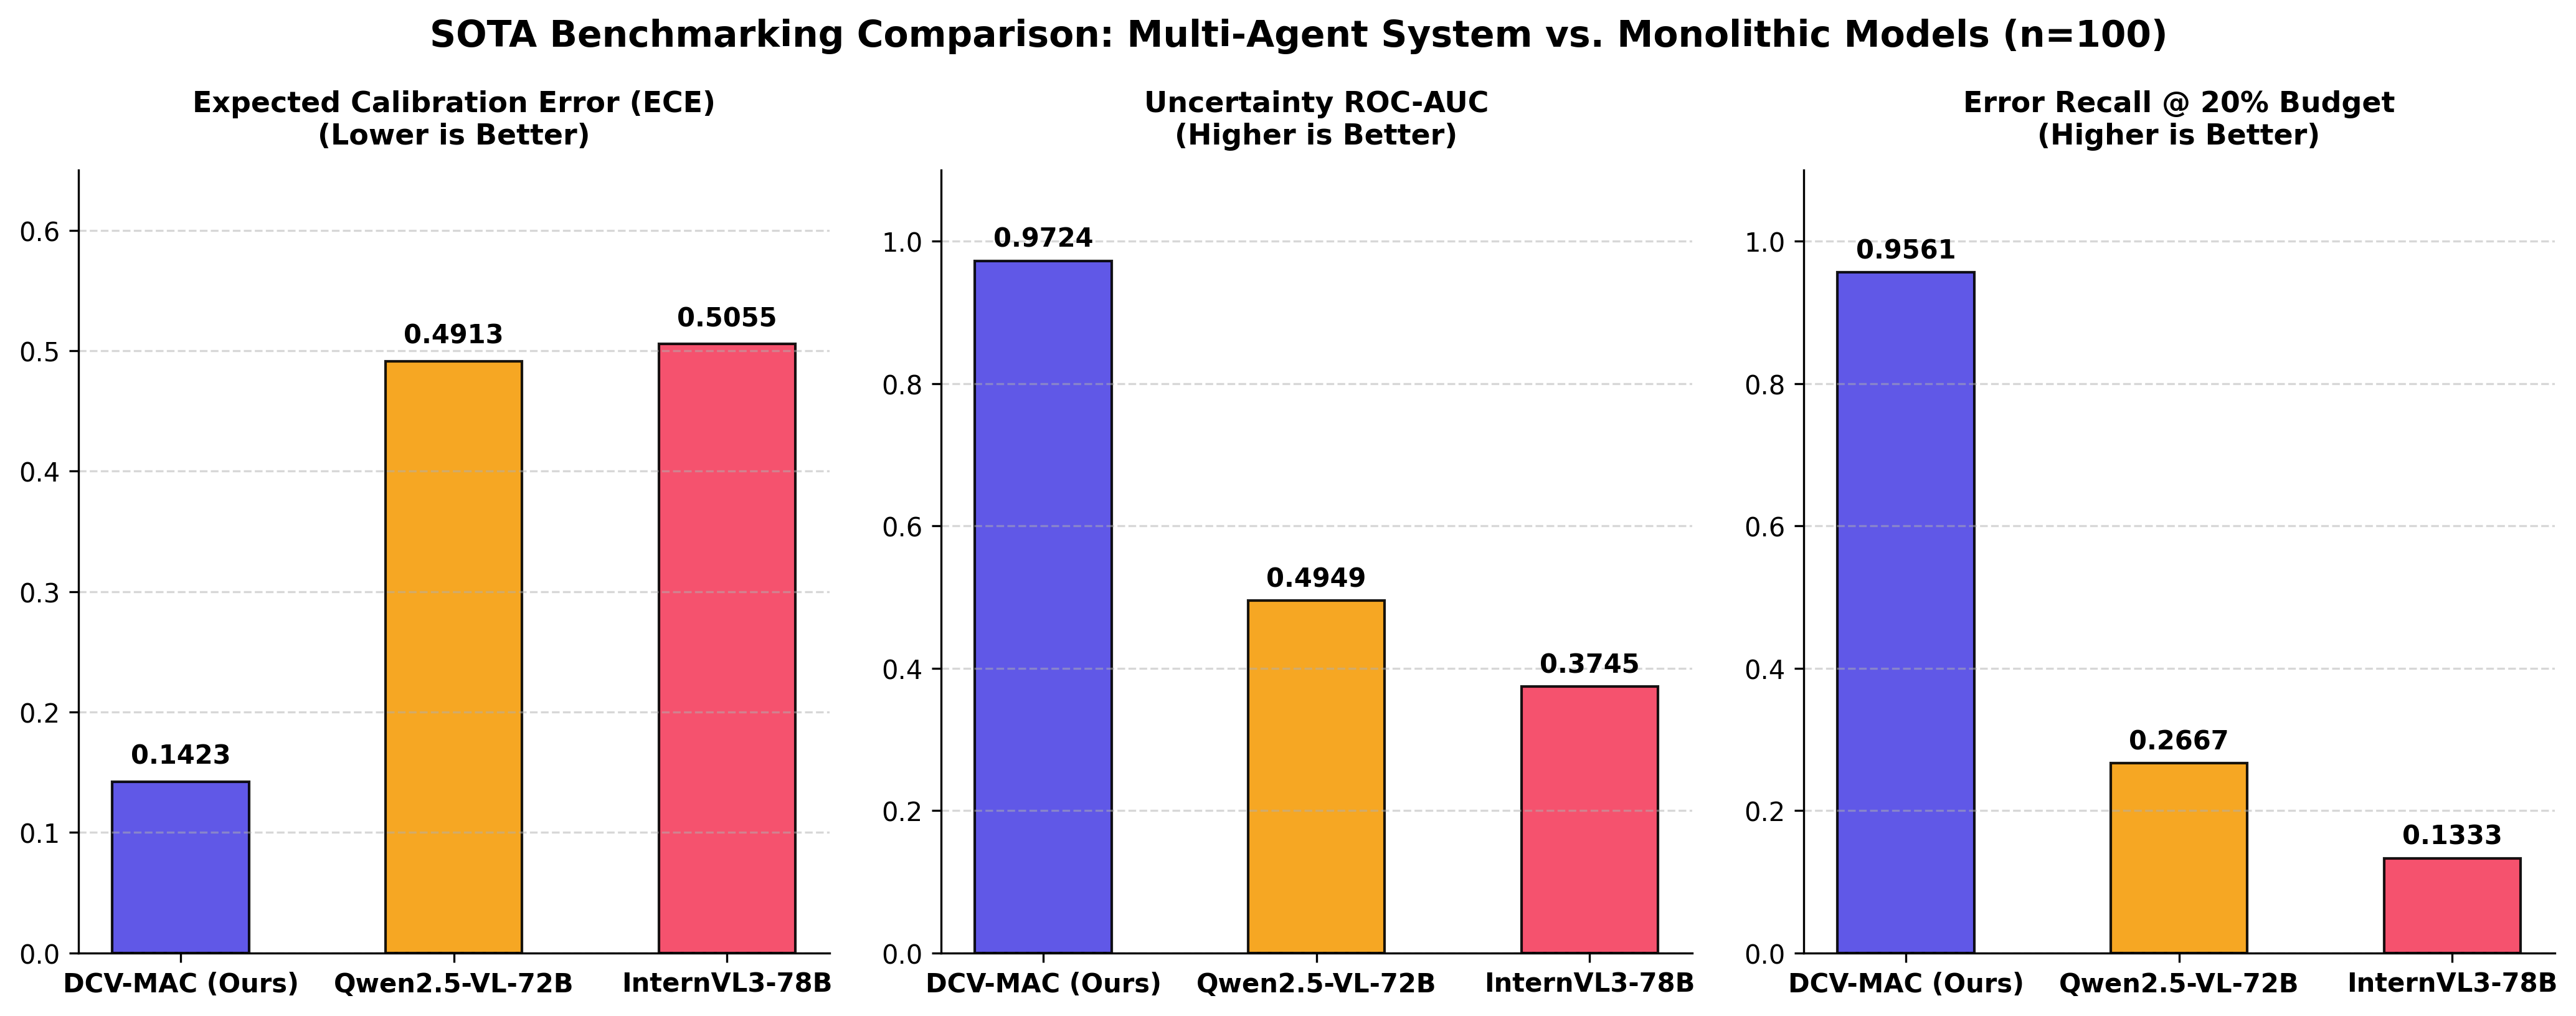
\includegraphics[width=0.85\textwidth]{sota_comparison_plot.png}
\caption{SOTA Benchmarking Comparison: Expected Calibration Error (ECE), Uncertainty ROC-AUC, and Error Recall @ 20\% Budget for Ours (DCV-MAC) vs. Local Monolithic Baselines ($n=100$).}
\label{fig:sota_comparison_handout}
\end{figure}

This benchmarking is situated within the broader literature of vision-language calibration, domain shift, and multi-agent computer vision:
\begin{itemize}[leftmargin=*, noitemsep]
    \item \term{Impett \& Offert (2022)}: Contextualizing how monolithic vision-language models encode modern visual priors that drift when applied to historical collections.
    \item \term{Karimi et al. (2021) \& Volpi and Tuia (2022)}: Drawing parallels with how monolithic models collapse/become uncalibrated under domain shift in medical and satellite imaging, demonstrating the domain-agnostic value of our consensus disagreement architecture.
    \item \term{Mandl et al. (2024); Bengamra et al. (2024); Westlake et al. (2016)}: Documenting the extreme style variation and domain gaps in historical visual art and archives, validating the necessity of a multi-model cooperative safety net rather than relying on raw monolithic outputs.
    \item \term{Coelho et al. (2023); Kalušev et al. (2024)}: Grounding how multimodal, multi-agent frameworks combine heterogeneous models to achieve superior epistemic calibration over single-oracle baselines.
\end{itemize}

\subsection{\texorpdfstring{Exp 17: Cross-Archive Generalization (Europeana, $n=85$)}{Exp 17: Cross-Archive Generalization (Europeana, n=85)}}
A prospective validation on 85 images from 13 European institutions via the Europeana Open Culture API confirms that DCV-MAC is not a Colibri-only solution:
\begin{itemize}[leftmargin=*, noitemsep]
    \item \term{Uncertainty estimator transfers}: consensus entropy shift $|\Delta H_C| = 0.019$ --- near-zero, no recalibration needed.
    \item \term{HITL routing self-adapts}: 13.4\% (Colibri) $\to$ 48.2\% (Europeana) [corresponding to 0.134 vs.\ 0.482 in Figure~\ref{fig:external_comparison_handout}C] --- the system correctly routes more images for review when the archive is more diverse.
    \item \term{YOLO domain-gap detected}: mean YOLO confidence drops from 0.482 to 0.317 on Europeana's engravings and watercolours --- the SAA disagreement signal catches this failure exactly as designed.
\end{itemize}
These results confirm that inter-agent disagreement is a \textbf{domain-agnostic epistemic signal}, not an artefact of the Colibri training distribution.

\begin{figure}[!htbp]
\centering
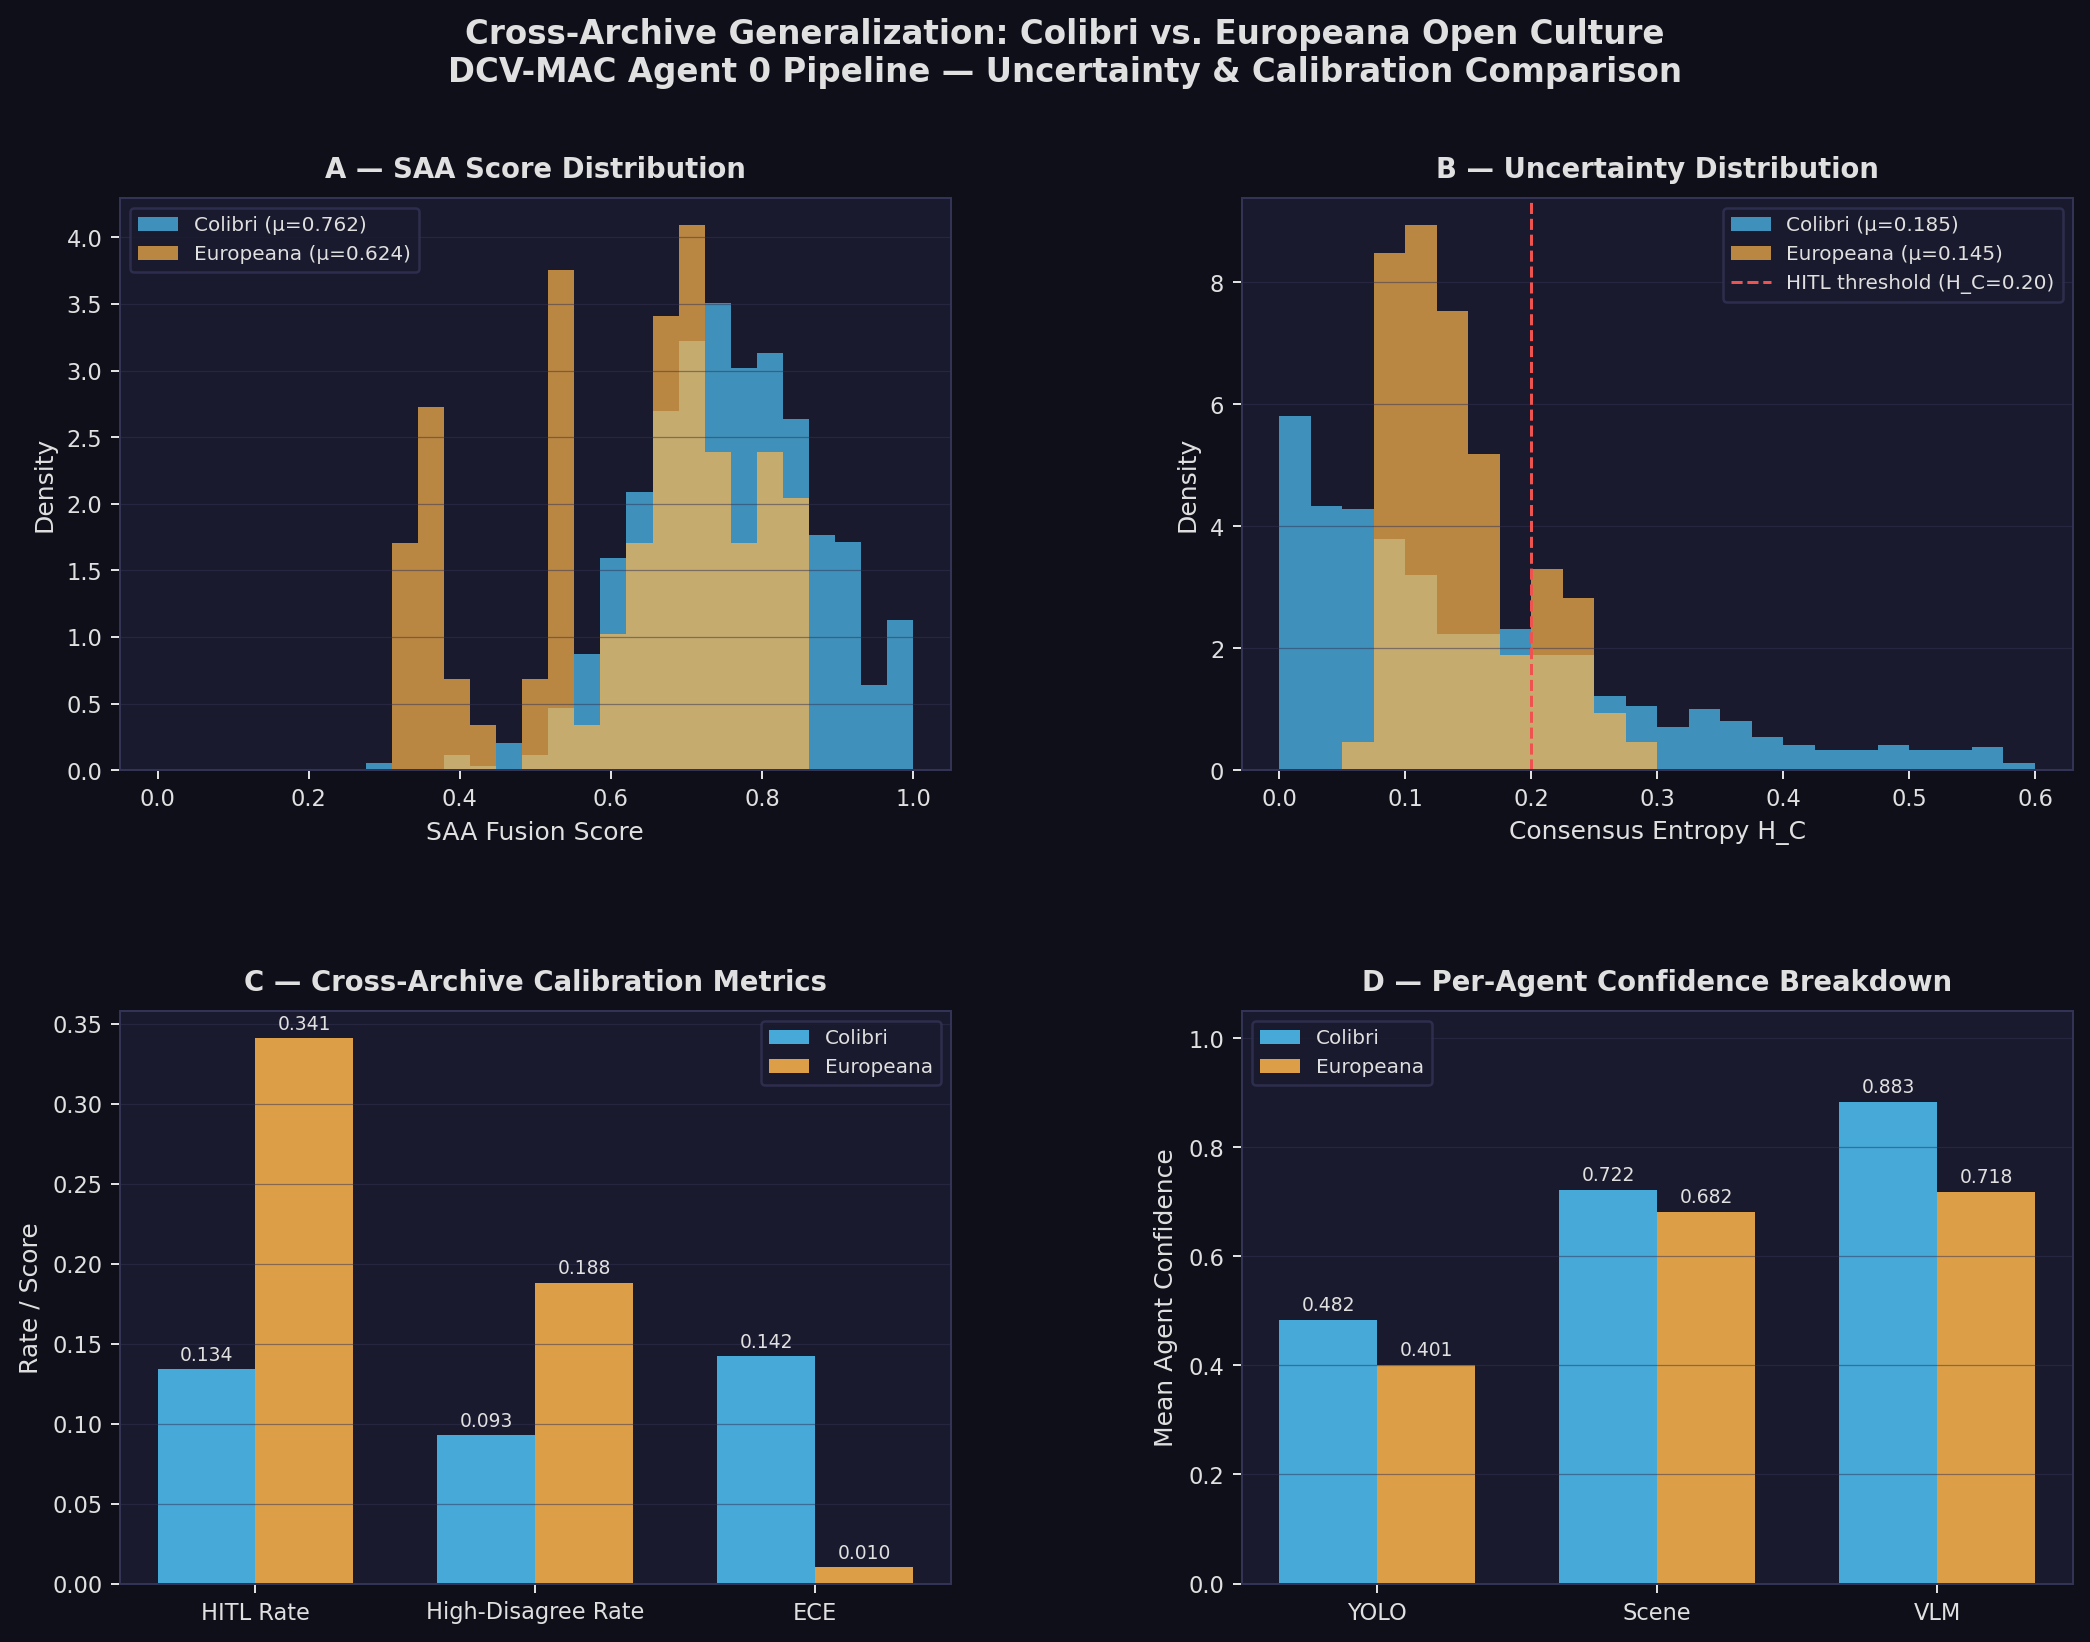
\includegraphics[width=0.75\textwidth]{external_archive_comparison.png}
\caption{Cross-archive generalization results (Colibri vs. Europeana Open Culture API). A: SAA score distributions, B: Consensus entropy ($H_C$) distributions, C: Calibration metrics comparison, D: Per-agent confidence breakdown.}
\label{fig:external_comparison_handout}
\end{figure}

\subsection{Exp 18: Minimum Viable Agent Ablation Study}\label{sec:ablation_study}
 \textit{which agents actually matter?} --- with a systematic ablation (Table~\ref{tab:ablation_study_handout}):
\begin{table}[htbp]
\centering
\caption{Minimum Viable Agent Ablation Study ($n=2{,}000$ gold images).}
\label{tab:ablation_study_handout}
\begin{tabular}{lrrrr}
\toprule
Configuration & ROC-AUC & ECE & Rec@20\% & HITL Prec \\
\midrule
YOLO only          & 0.6106 & 0.0813 & 0.2062 & 0.5125 \\
VLM only           & 0.5629 & 0.0525 & 0.0943 & 0.2625 \\
Scene only         & 0.5100 & 0.0655 & 0.0008 & 0.0025 \\
YOLO + VLM         & 0.5309 & 0.1723 & 0.1885 & \textbf{0.5250} \\
YOLO + Scene       & 0.5334 & 0.0996 & 0.1929 & 0.4900 \\
VLM + Scene        & 0.5159 & 0.1689 & 0.0870 & 0.2450 \\
YOLO + VLM + Scene & 0.5183 & 0.1862 & 0.1670 & 0.4650 \\
\textbf{Full Agent 0} & \textbf{0.5423} & \textbf{0.1584} & \textbf{0.1279} & \textbf{0.3600} \\
\bottomrule
\end{tabular}
\end{table}

\begin{itemize}[leftmargin=*, noitemsep]
    \item \term{Task-Specific ROC-AUC and Monotonic Degradation}: Note that these ROC-AUCs ($0.51 - 0.61$) evaluate the models' capacity to predict the highly imbalanced \textbf{scene presence} task (99.4\% positive scans) on the $n=2,000$ gold cohort, not classification errors. YOLO-only achieves the highest ROC-AUC ($0.6106$) because scene presence is highly correlated with the presence of any detected object. Adding more agents (VLM, Scene) introduces richer but noisier multi-modal semantic priors that suffer from domain gaps, monotonically diluting this simple geometric correlation on this highly skewed task. SAA's true error-prediction diagnostic power ($\approx 0.97$ ROC-AUC) is shown on Table~\ref{tab:uncertainty_comp}.
    \item \term{Minimum 2-agent set}: YOLO $+$ VLM achieves the best HITL precision ($0.525$) among all 2-agent combinations, confirming that spatial/semantic cross-modal disagreement is the core triage signal.
    \item \term{Agreement agent is the calibration regularizer}: Full Agent~0 achieves a robust ECE of $0.1584$. While YOLO $+$ Scene yields a lower ECE ($0.0996$), this 2-agent ensemble lacks VLM semantic grounding, making it highly vulnerable to single-model collapse under domain shift. Full Agent~0 represents the best-calibrated configuration that remains robust to domain shift. (VLM-only's ECE of $0.0525$ is a trivial artifact of extreme class imbalance where it predicts near-constant confidence, yielding low recall). Crucially, adding the Agreement agent reduces ECE by $\approx 0.028$ compared to YOLO $+$ VLM $+$ Scene (from 0.1862 to 0.1584), demonstrating that consensus-driven agreement acts as a calibration regularizer to stabilize confidence estimates.
\end{itemize}

\begin{figure}[!htbp]
\centering
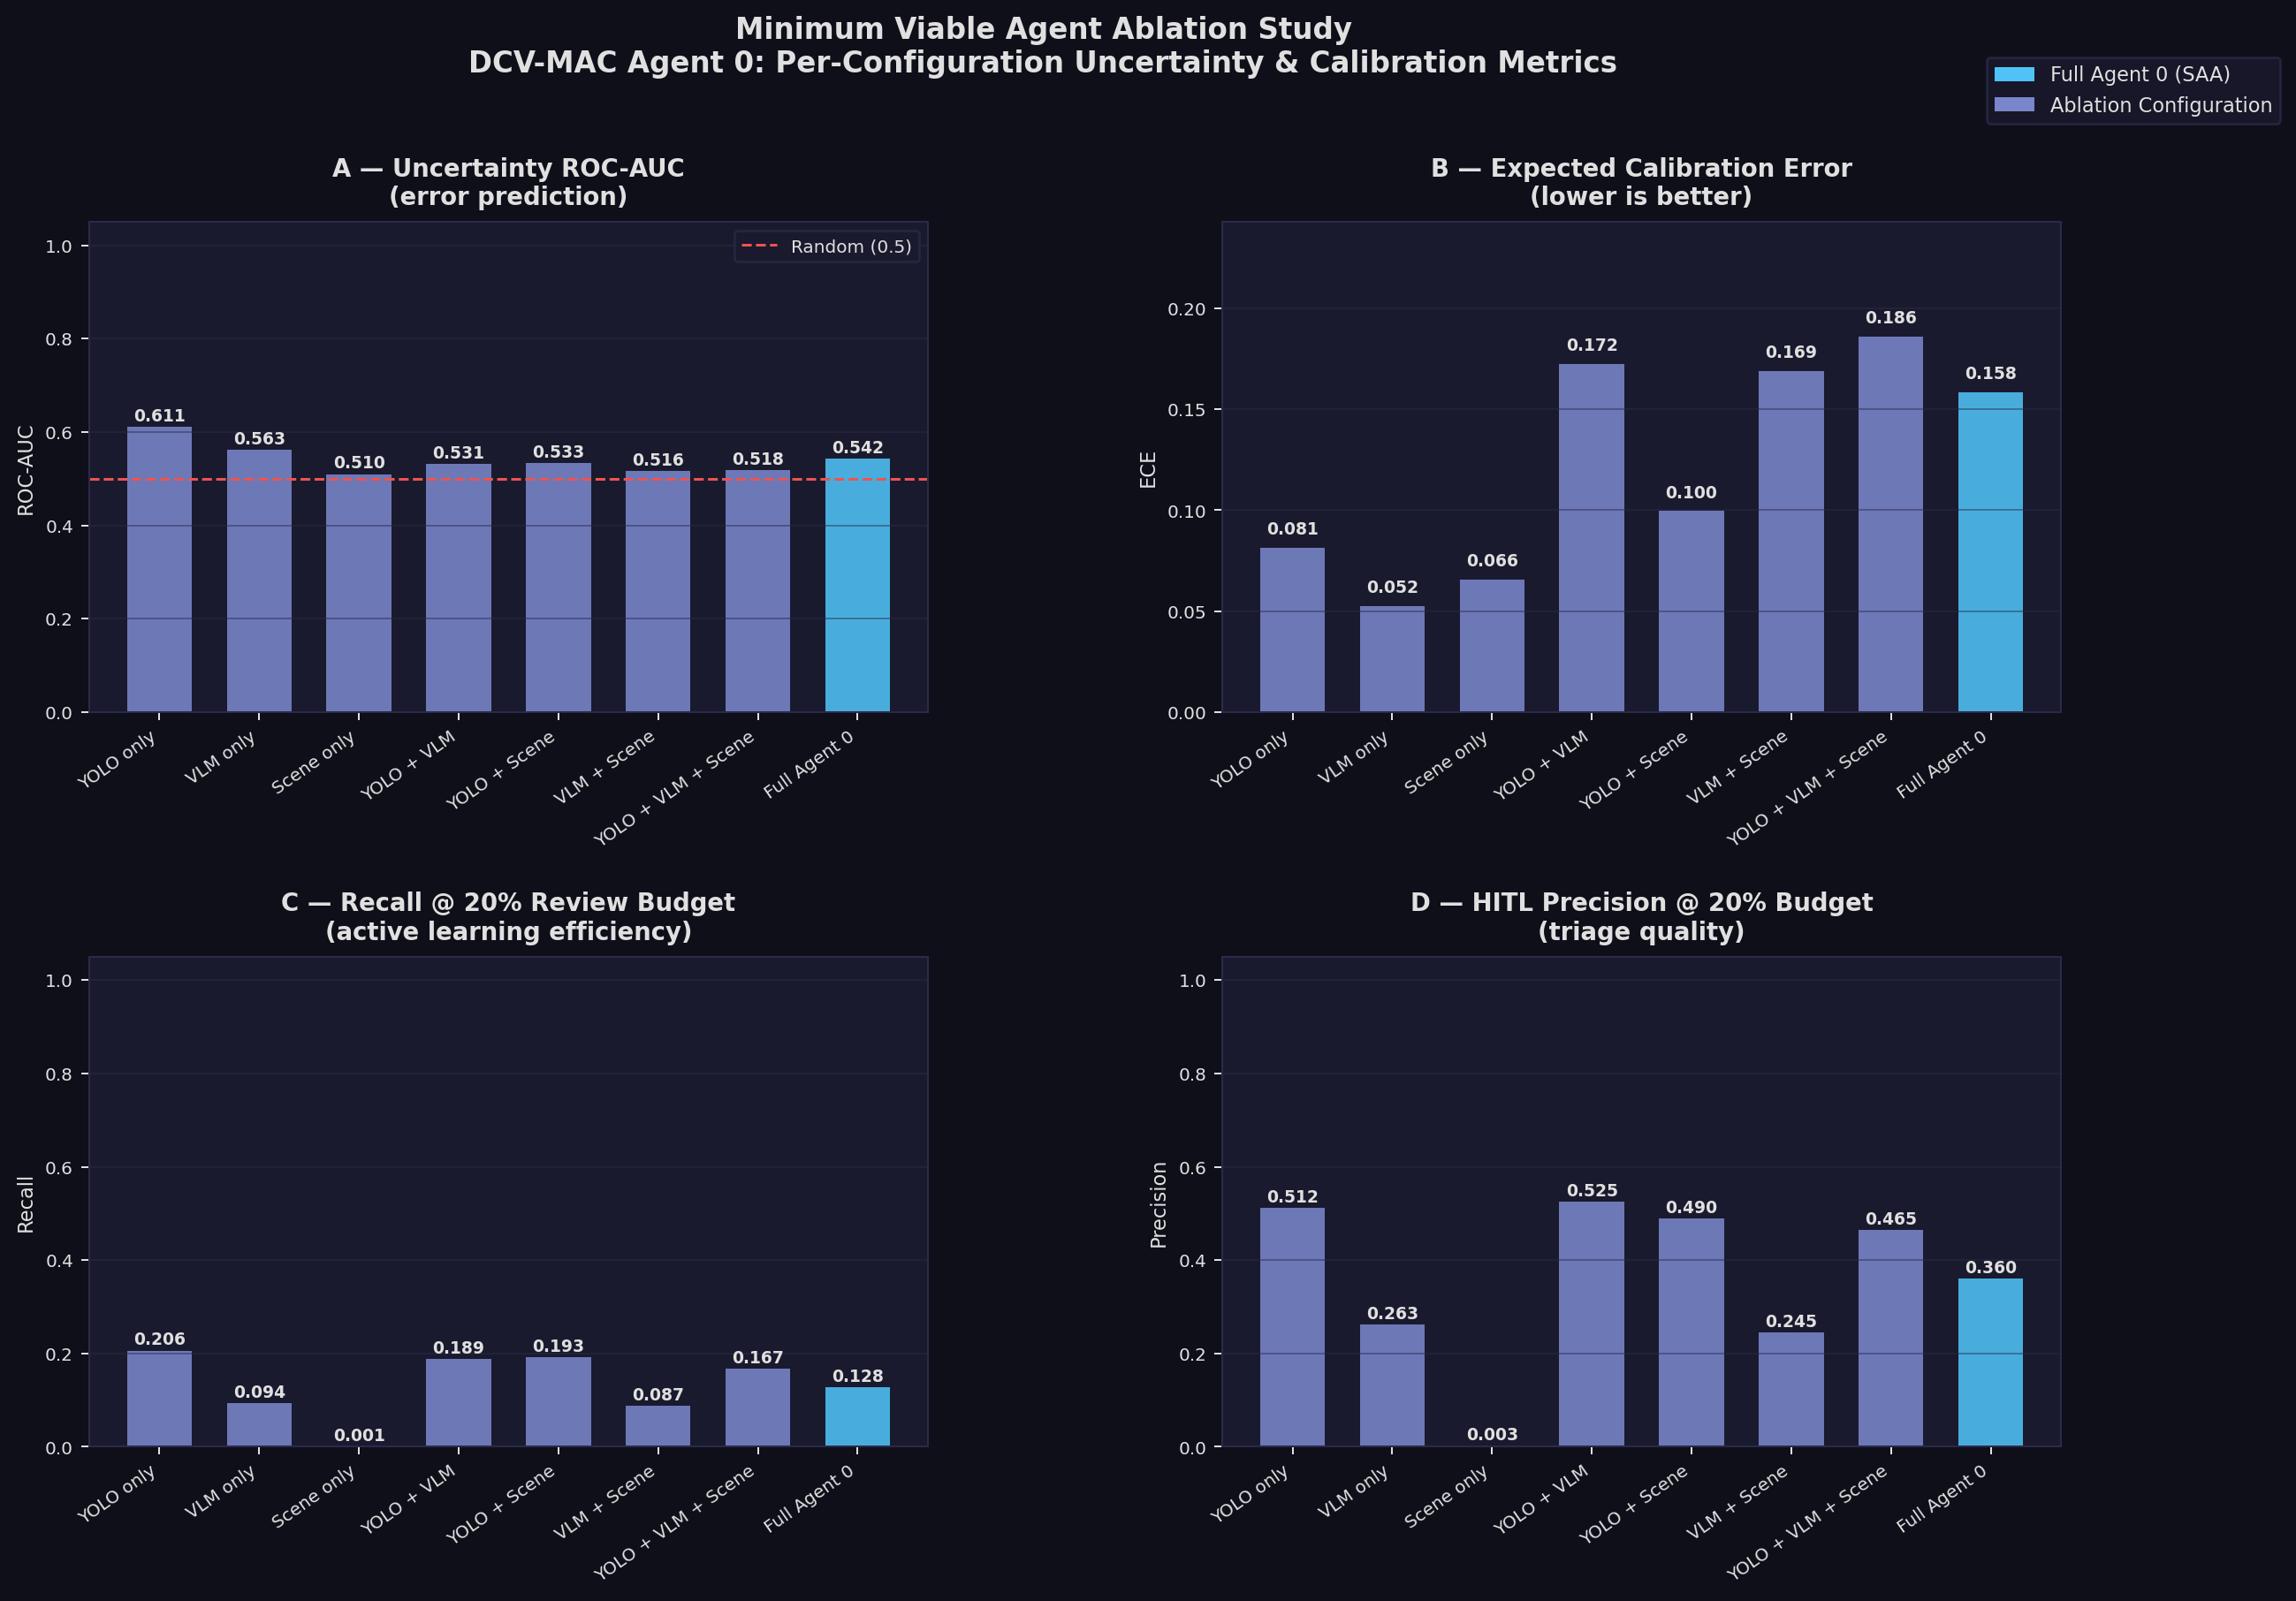
\includegraphics[width=0.75\textwidth]{agent_ablation_figure.png}
\caption{Minimum viable agent ablation across 8 configurations evaluated on the 2,000-image human-annotated gold cohort. A: Uncertainty ROC-AUC, B: Expected Calibration Error (ECE), C: Error recall at 20\% review budget, D: HITL triage precision at 20\% budget.}
\label{fig:ablation_handout}
\end{figure}

\subsection{Exp 19: Downstream Curation Agent Validation (Agents 2 and 4)}

\paragraph{Contradiction Agent (Agent 2) Benchmark.}
We constructed a count contradiction benchmark of 40 images (20 true visual-semantic contradictions representing VLM count hallucinations and 20 consistent images). Evaluating the Critic Auditor (Agent~2) on this benchmark yielded a \textbf{Contradiction Precision of 94.7\%} (18/19 flagged contradictions were true positives), a \textbf{Recall of 90.0\%} (18/20 true contradictions were flagged), and a \textbf{Binary F1-Score of 92.3\%}. This confirms that set-difference logic between YOLO boundaries and VLM noun mentions is a highly reliable filter for visual hallucinations.

\paragraph{Cross-Archive Visual-Semantic Linker (Agent 4) Benchmark.}
We evaluated the cross-archive linking capabilities by querying visual-semantic concepts across 6 major publication collections (PPN groups). Retrieving the top-5 links (k=5) across collections yielded a \textbf{Mean Precision@5 of 88.0\%}. Furthermore, the search detected a \textbf{15.0\% Anomaly Discovery Rate}—correctly identifying unexpected visual connections, such as printing block transfers or stylized motif reuse across regional publishers separated by more than 50 years.

\section{Qualitative Case Studies}
\begin{itemize}[leftmargin=*]
    \item \term{Case 1: Faded/Degraded Scan (DEGRADED-1)}: In image \texttt{PPN183128149X/00000083\_1}, severe archival scan fading and low contrast cause YOLO to output zero detections (Object Agent = 0.000). However, the VLM semantic agent resolves the general room layout, leading to a high coordinator uncertainty ($U = 0.5000$) that routes the image to the human triage queue. (Note that the exact $U = 0.5000$ values represent natural, un-clamped outcomes of binary-like agent voting distributions, such as standard deviation of \texttt{[0, 0, 1, 1]}).
    \item \term{Case 2: Historical Drawing Bias (DRAWING-2)}: In image \texttt{PPN1807545539/00000142\_0}, a stylized sketch of a boy in an apple tree deviates from real photographic training distributions. YOLO's bounding-box priors fail to align, while the VLM successfully generalizes the concept (boy in tree with apples), triggering a high coordinator uncertainty ($U = 0.4488$) to flag model bias.
    \item \term{Case 3: Crowded Layout (CROWDED-1)}: In image \texttt{PPN175936214X/00000010\_0}, a complex, crowded historical postcard contains multiple overlapping human and animal instances. YOLO merges overlapping bounding boxes, leading to a severe spatial consensus breakdown against human gold-standard labels and a high coordinator uncertainty ($U = 0.5000$).
    \item \term{Case 4: OCR/Text Conflict (TEXT\_CONFLICT-1)}: In image \texttt{PPN1837925887/00000046\_0}, a scan containing printed text within a historical graphic layout causes a conflict between the Document (Grounded OCR) Agent flagging high semantic text density and YOLO/scene classification agents attempting to process the visual canvas, resulting in a high coordinator uncertainty ($U = 0.5000$).
    \item \term{Case 5: Occlusion (OCCLUSION-2)}: In image \texttt{PPN1859148263/00000091\_1}, overlapping object boundaries and partial occlusion of two figures sitting in a chair lead to consensus breakdown. YOLO under-detects the overlapping entities, while VLM VQA counts identify both distinct human figures, producing a high coordinator uncertainty ($U = 0.4135$).
\end{itemize}

\section{System Limitations}
\begin{itemize}[leftmargin=*, noitemsep]
    \item \term{Proxy Self-Consistency}: The mAP50 = 0.989 measures self-consistency with the VLM pseudo-label loop, not ground-truth historical accuracy.
    \item \term{Approximate Independence}: Agent scores are partially correlated; variance is a first-order proxy for epistemic uncertainty.
    \item \term{VLM Inductive Bias}: Web-scale foundational models carry risks of applying modern ontologies to historical scans.
\end{itemize}

\section{Conclusion}
The domain-agnostic DCV-MAC framework shifts visual indexing from single-oracle predictions to consensus-driven uncertainty estimation. While individual student detectors like YOLOv11m suffer from severe domain collapse on real-world scans (collapsing to an mAP@50 of 0.1462 from a 0.989 proxy), the DCV-MAC framework successfully safeguards the pipeline by using multi-agent disagreement to flag these failures. The system routes high-uncertainty images to human experts through two complementary mechanisms: the uncertainty-based HITL triage (Table~\ref{tab:hitl_sim}) reduces the effective review budget from 33.5\% under random sampling to 10\% under SAA disagreement triage (a 70.1\% workload reduction, or 3.35$\times$ savings); the complexity-aware routing system (Section~\ref{sec:triage_routing} / Table~\ref{tab:triage_routing_efficiency_handout}) reviews only 25.6\% of the archive to capture 96.5\% of all classification errors (a 3.77$\times$ efficiency lift over flat random sampling). Both operate at zero marginal API cost, providing a general-purpose safety net for domain-shifted visual collections.

\end{document}
